\documentclass[oneside,12pt, numbered]{book}


%\usepackage[Lenny]{fncychap}
\usepackage{a4wide}
\usepackage[francais]{babel}
\usepackage[utf8]{inputenc}
\usepackage[T1]{fontenc}
\usepackage{enumitem}
\usepackage{xcolor}
\usepackage{shorttoc}

\usepackage{url}
\usepackage[autolanguage]{numprint}
\usepackage{float}
 \usepackage{hyperref}
\usepackage{frcursive}
\usepackage{icomma}
\usepackage{graphicx}
\usepackage{listings}
\usepackage[]{siunitx}
\usepackage{textcomp}
\usepackage{geometry}
 \geometry{
 a4paper,
 left=19mm,
 right=19mm,
 top=21mm,
 bottom= 18mm,
 }

\hypersetup{
colorlinks=true,
linkcolor=blue,
citecolor=blue,
filecolor=black,
urlcolor=black
}

\usepackage[explicit]{titlesec}
\usepackage{lmodern}
\usepackage{color}
\newlength\chapnumb
\setlength\chapnumb{3cm}


\titleformat{\chapter}[block] 
{\sffamily}{}{0pt} {
\parbox[b]{\chapnumb}{
\fontsize{90}{80}\selectfont\thechapter}
\parbox[b]{\dimexpr\textwidth-\chapnumb\relax}{
\raggedleft
\hfill{\Huge\sffamily#1}\\
\rule{\dimexpr\textwidth-\chapnumb\relax}{0.8pt}
}
}

\titleformat{name=\chapter,numberless}[block]
{\sffamily}{}{0pt}
{\parbox[b]{\chapnumb}{%
\mbox{}}%
\parbox[b]{\dimexpr\textwidth-\chapnumb\relax}{
\raggedleft
\hfill{\Huge\sffamily#1}\\
\rule{\dimexpr\textwidth-\chapnumb\relax}{0.8pt}}}
    


%%configuration de listings
\lstset{
language={[Sharp]C},
}

\setlength{\parindent}{0cm}

\graphicspath{{images/}}
\def\Titre{La technologie dans le cadre de l'entraînement d'un coureur de haut niveau}
\def\title{La partie invisible de la performance sportive révélée par la technologie} %Application et expérimentation au 400m

\def\Auteur{Joan Medjid}
\def\Version{0.1}
\def\Date{\today}

\usepackage{fancyhdr}
\pagestyle{fancy}
\fancyfoot{}
\fancyhead[L,RO]{\bfseries\thepage}
\fancyhead[LO]{\bfseries\nouppercase{\rightmark}}


\renewcommand{\thesubsubsection}{\alph{subsubsection})}
\renewcommand{\appendixautorefname}{Annexe}

\setcounter{secnumdepth}{3}




\begin{document}

\begin{titlepage}
        \begin{center}

            \begin{figure}
            \centering
            \vspace{30pt}
              
\includegraphics[width=0.5\textwidth]{logo-nanterre}\\[1.5cm]
            \end{figure}
            
            
            {\LARGE Master MIAGE}\\[0.5cm]
            {\LARGE Mémoire de fin d'étude}\\[2cm]
            
            \rule{\linewidth}{0.6mm} \\[0.4cm]
            { \huge \bfseries \title \\[0.4cm] }
            \rule{\linewidth}{0.6mm} \\[0.4cm]
   
            \begin{figure}[H]
             \centering
            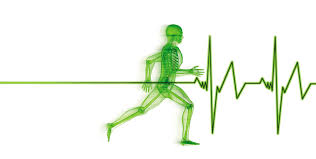
\includegraphics[scale=1]{images/analyse2.jpg}
            \end{figure}
            
            \vspace{0.4cm}
            
            \large{\emph{Réalisé par :}}\hspace{30ex}\large{\emph{Encadré par :}}
            

            \hspace{2ex} \LARGE{Joan \textsc{Medjid}}\hspace{12ex}\hspace{1ex}\LARGE{Lom Messan \textsc{Hillah}}\\[2cm]
            
            
             \Large{Année universitaire 2017-2018}
        
        \end{center}
    \end{titlepage}
        

    \frontmatter
   
        \chapter*{Résumé}
\addcontentsline{toc}{chapter}{Résumé}
\markboth{Résumé}{Résumé}
\label{chap:resume}
%\minitoc



Les relations entre certains aspects de la partie invisible de la performance comme la lactatémie, la glycémie, la fréquence cardiaque et l'oxymétrie de pouls ont été étudié chez 3 athlètes à la suite de courses de 400 mètres. Les mesures ont étés effectuées dans les 5 minutes suivant l'achèvement de l'effort avec des outils spécifiques. Les données recueillies ont ensuite été analysées.. \\

La découverte majeure de cette étude à été révélée par l'analyse des valeurs de la lactatémie. \\

Chez les 3 sujets, l'écart de lactatémie entre la valeur avant la course et celle après était très fortement lié à la performance réalisée (r=-
-0.97 avec P <0,05). Plus cet écart était important, meilleure était la performance de l'athlète relativement à ces autres performances. Cela indique alors qu'une des clés de la performance au 400 mètres est d'être capable de produire de grandes quantités de lactate tout en ayant des valeurs de lactatémie très basse avant la course.\\

Parallèlement à cela, la modification de l'échauffement d'un des sujets à la suite de l'analyse de taux anormaux de lactatémie, lui a permis d'améliorer considérablement ses performances (d'environ 2 secondes).\\

Ces résultats suggèrent que l'analyse de la partie invisible de la performance et notamment de la lactatémie permet de mieux comprendre la performance et dans certains cas, de l'améliorer.

        
%%% Local Variables: 
%%% mode: latex
%%% TeX-master: "memoire"
%%% End:
        \chapter*{Introduction}
\addcontentsline{toc}{chapter}{Introduction}
\markboth{Introduction}{Introduction}
\label{chap:introduction}

Le sport est un domaine d'intérêt où les humains ont toujours essayé de repousser les limites. Chaque jour un record est battu et la frontière de la performance est redéfinie. \\

Certaines découvertes ont malheureusement ouvert la porte à la tricherie, mais d’autres ont permis de comprendre comment obtenir de meilleurs résultats sans avoir recours à des substances interdites.\\

C'est notamment le cas de la technologie qui tient aujourd'hui une place prépondérante dans le monde du sport. Elle est utilisée en permanence, que ce soit pour augmenter l'efficacité des matériaux ou encore pour analyser des performances, dans le but de courir toujours plus vite ou de sauter toujours plus haut.\\

Toutefois, bien que la technologie permette d'analyser la performance, celle-ci est tellement complexe que sa compréhension n'est généralement que partielle.\\

En effet, lorsque nous terminons une course, le seul indicateur de performance auquel nous ayons accès est la partie visible de la celle-ci, représentée par le chronomètre, la distance ou encore le classement. Cependant, ces résultats ne sont que des nombres et ne signifient finalement rien. Nous ne connaissons en réalité pas du tout les effets que cet effort a produit sur notre organisme. \\

L'objectif de cette étude est donc de répondre à ce besoin de compréhension de la performance en s'intéressant à divers outils utilisables dans le quotidien d'un athlète et qui permettraient de rendre visible la partie invisible de la performance.\\

L'analyse des données récoltées grâce à ces outils pourrait permettre de mettre en lumière des axes d'amélioration dans l'entraînement de l'athlète, mais aussi des stratégies à adopter lors de l’approche des grandes compétitions.\\

C'est donc la recherche de l'amélioration des résultats qui anime l'analyse des composantes individuelles de la performance. En effet, dés lors que l'athlète et l'entraîneur sont capables d'isoler des zones sur lesquelles se concentrer à l'entraînement, le résultat final est susceptible d'être amélioré.\\

Étant athlète de haut niveau et pratiquant les disciplines de 400m et 400m haies, l'utilisation de tels outils pourrait réellement m'aider dans l'accomplissement de mon rêve et de l'objectif de ma vie : les jeux olympiques.\\



%%% Local Variables: 
%%% mode: latex
%%% TeX-master: "memoire"
%%% End:
        \chapter*{Contribution de ce mémoire}
\addcontentsline{toc}{chapter}{Contribution}
\markboth{Contribution}{Contribution}
\label{chap:contribution}

Pour mener à bien cette étude, je me suis intéressée à quatre facteurs physiologiques qui me paraissaient important pour être performant lors d'une course de 400 mètres : 
\begin{itemize}
    \item la lactatémie,
    \item la glycémie,
    \item la fréquence cardiaque,
    \item l'oxymétrie de pouls.\\
\end{itemize}


J'ai mesuré ces facteurs à l'aide d'outils spécifiques : 
\begin{itemize}
    \item un lactatomètre,
    \item un glucomètre,
    \item une montre cardio-fréquencemètre,
    \item un oxymètre de pouls.\\
\end{itemize}

Les mesures ont étés effectuées avant et après des courses de 400 mètres réalisées par 3 athlètes spécialistes de cette discipline. \\

Les données mesurées par les différents outils ont ensuite été analysées par un logiciel de statistiques pour en tirer des résultats intéressants. \\


        
%%% Local Variables: 
%%% mode: latex
%%% TeX-master: "memoire"
%%% End:
        \chapter*{Plan}
\addcontentsline{toc}{chapter}{Plan}
\markboth{Plan}{Plan}
\label{chap:plan}


Afin de répondre au mieux à la problématique, je définirai dans un premier temps la performance ainsi que les déterminants de celle-ci en athlétisme, que ce soient les facteurs physiologiques, l'environnement social de l'athlète, l'entraînement invisible ou encore les cotés physiques et psychologiques.\\

Dans un deuxième temps, je m’intéresserai à divers outils existants qui permettent de mesurer certains facteurs physiologiques et ainsi de mettre en lumière la partie invisible de la performance. \\

Je présenterai ensuite un état de la littérature existante sur le sujet, regroupant divers articles qui seront complémentaires à mon étude.\\

Enfin, dans une dernière partie, j'analyserai les données recueillies à travers des expérimentations sur différents athlètes afin de pouvoir conclure et répondre au problème posé.



        
%%% Local Variables: 
%%% mode: latex
%%% TeX-master: "memoire"
%%% End:
        \chapter*{Remerciements}
\addcontentsline{toc}{chapter}{Remerciements}
\markboth{Remerciements}{Remerciements}


Je tiens à remercier toutes les personnes qui ont participé de prés ou de loin au bon déroulement de mon mémoire de fin d'étude. \\

Mes sincères remerciements à mon tuteur, \textbf{Mr Lom Messan Hillah}, pour le temps et l'intérêt qu'il m'a accordé afin que je produise le meilleur travail possible mais aussi pour tout ce qu'il m'a enseigné durant ces cinq dernières années.\\

Mes remerciements également à mon entraîneur et à mon kinésithérapeute qui m'ont guidée, conseillée et ont répondu à toutes mes attentes concernant la réalisation de ce mémoire.\\

Enfin je remercie tous \textbf{les professeurs de la MIAGE de Nanterre} pour leur implication et les connaissances qu'ils m'ont transmises durant ces années d'études à l'Université.
        \shorttableofcontents{Sommaire}{0}

        \newpage
        
        \listoffigures

        \chapter*{Glossaire}
\addcontentsline{toc}{chapter}{Glossaire}
\markboth{Glossaire}{Glossaire}
\label{chap:glossaire}
%\minitoc


\textbf {Fréquence cardiaque} Nombre de battements cardiaques par unité de temps. \\


\textbf {Glucose} Principale source d'énérgie de notre organisme.\\

\textbf {Glycémie} Taux de glucose dans le sang.\\

\textbf {Indice glycémique} Critère de classement des aliments contenant des glucides, basé sur leurs effets sur la glycémie durant les deux heures suivant leur ingestion.\\

\textbf{Lactate} Sel majoritairement produit par les muscles, les globules rouges et les cellules cérébrales au cours de la production d’énergie anaérobie. \\

\textbf {Lactatémie} Concentration de lactate dans le sang. \\

\textbf {Oxymétrie de pouls} ou \textbf{Saturation pulsée en oxygène} Quantité d’oxygène qui circule dans le sang.\\

\textbf{Physiologique} Relatif à l'activité du corps humain (fonctionnement mécanique, physique et biochimique).\\ 

\textbf{Volume d’Oxygène Maximal} Quantité maximale d'oxygène que l'organisme est capable d'absorber lors d'un effort physique. \\ 


        
%%% Local Variables: 
%%% mode: latex
%%% TeX-master: "memoire"
%%% End:
        \chapter*{Liste d’abréviations, de sigles et de symboles}
\addcontentsline{toc}{chapter}{Liste d’abréviations, de sigles et de symboles}
\markboth{Liste d’abréviations, de sigles et de symboles}{Liste d’abréviations, de sigles et de symboles}
\label{chap:abreviation}
%\minitoc

\textbf{bpm} battement par minute \\

\textbf{FCM} fréquence cardiaque maximale\\

\textbf{g/l} gramme par litre \\

\textbf{IG} indice glycémique \\

\textbf{kg} kilogramme \\

\textbf{km/h} kilomètre par heure\\

\textbf{l} litre \\

\textbf{m} mètre \\

\textbf{mg/dl} milligramme par décilitre \\

\textbf{min} minute \\

\textbf{mmol} millimole \\

\textbf{mmol/l} millimole par litre\\

\textbf{nm} nanomètre\\

\textbf{s} seconde \\

\textbf{SPO2} saturation pulsée en oxygène\\

\textbf{VO2max} volume d'oxygène maximal \\

\textbf{W} watt \\       
%%% Local Variables: 
%%% mode: latex
%%% TeX-master: "memoire"
%%% End:
        \chapter*{Contexte}
\addcontentsline{toc}{chapter}{Contexte}
\markboth{Contexte}{Contexte}
\label{chap:contexte}

Le thème de ce mémoire a été très facile à trouver car il s'est tout naturellement orienté vers un sujet liant mes deux passions qui sont l'athlétisme et l'informatique. Toutefois, la problématique à quant à elle été plus compliquée à formuler. Beaucoup de pistes étaient intéressantes à explorer, mais aucune d'entre elles ne résolvaient un réel problème, ou bien elles étaient trop compliquées à résoudre.\\

Mon tuteur, Mr Lom Hillah, m'a alors suggéré d'effectuer une étude de terrain auprès des athlètes de mon club d'athlétisme afin de connaître leurs besoins. \\

Beaucoup d'entre eux m'ont fait part de leur souhait de pouvoir améliorer leurs performances grâce à l'utilisation de la technologie et notamment de divers outils informatiques. Cet axe était également une de mes premières idées, mais en en faisant part à mon tuteur mais également à mon entraîneur, je me suis rendu compte que cela serait trop compliqué à étudier. En effet, pour pouvoir déterminer si un outil permet réellement d'améliorer une performance il faudrait le tester sur un échantillon d'athlètes réalisant la même discipline, dans les mêmes conditions. Cela implique que pour chacun des athlètes, tous les paramètres doivent être identiques : les entraînements précédents, le sommeil, l'alimentation, le coté psychologique etc. Or cela demande un réel cadre de recherche et je ne dispose pas d'assez de temps ni de moyens pour mener une étude de cette ampleur. \\

Un autre besoin qui a été évoqué est celui de pouvoir prédire le pic de forme, c'est à dire le moment où notre potentiel est porté à son maximum. J'ai réfléchi à ce sujet et j'en suis venu au fait que pour pouvoir prédire un pic de forme, mais également améliorer les performances, il fallait tout d'abord comprendre les courses et les entraînements précédents. Cela passe non seulement par l'étude de la partie visible de la performance c'est à dire les différents temps de passage ou encore le chronomètre final, mais aussi et surtout, par l'étude de sa partie invisible. Cette partie invisible de la performance est déterminée entre autres par différents aspects physiologiques comme la lactatémie, la glycémie, l'oxymétrie ou encore la fréquence cardiaque de l'athlète, mais n'est que très peu étudiée par les athlètes et entraîneurs.\\


%%% Local Variables: 
%%% mode: latex
%%% TeX-master: "memoire"
%%% End:
        \chapter*{Problématique}
\addcontentsline{toc}{chapter}{Problématique}
\markboth{Problématique}{Problématique}
\label{chap:problématique}

A la suite de cette réflexion, la problématique la plus pertinente qui a émergé est : \\

\vspace{10pt}

\textbf{La technologie permet-elle de rendre visible la partie invisible de la performance ?}\\

\vspace{10pt}

La technologie et notamment divers outils de mesure sanguine pourraient en effet permettre de mesurer certains facteurs de la partie invisible de la performance.\\  

L'ensemble des données collectées seraient ensuite analysées par des logiciels d'analyse de données afin de révéler différents aspects qui ne seraient pas visible au premier abord et notamment les effets de l'effort produit sur l'organisme. \\

L'analyse de la partie invisible de la performance pourrait ainsi devenir un moyen courant de contrôle et d'optimisation de l'entraînement, de récupération, mais aussi de compréhension des performances réalisées en compétition.\\

En fonction des résultats obtenus, l'entraîneur pourrait déterminer pourquoi l'athlète a été plus performant sur une course plutôt qu'une autre et ainsi adapter les entraînements pour qu'ils correspondent à la physiologie et aux besoins de chaque athlète.\\

En outre, lorsque nous serons capable de comprendre nos performances, nous pourrons peut être par la suite améliorer une partie de la performance, ce qui est l'objectif de tout athlète.




%%% Local Variables: 
%%% mode: latex
%%% TeX-master: "memoire"
%%% End:
    
    \mainmatter
  
         \chapter{La performance en athlétisme}
\label{part:performance}


Avant de s'intéresser à la problématique posée, nous  allons dans un premier temps définir tous les concepts de ce mémoire et notamment la performance sportive ainsi que ses déterminants.\\

    \section {Qu'est ce que la performance sportive ?}
    
        \subsection{Définition de la performance}
        
            Selon Vladimir Platonov \cite{platonov88}, scientifique dans le domaine des sciences du sport, « la performance sportive exprime les possibilités maximales d'un individu dans une discipline à un moment donné de son développement ». \\
            
            Pour Francis Trilles \cite{trilles02}, c'est « l'aboutissement, le point final (ou intermédiaire) d'une série d'actions appelées préparation sportive. Elle constitue l'objectif d'un long processus d'entraînement. »\\
        
            Nous pouvons également dire que la performance sportive est le résultat d’adaptations motrices aux contraintes et possibilités d'une discipline. 
            Ces contraintes peuvent être d'ordre :
            \begin{itemize}
                \item réglementaires : par exemple au 400m en athlétisme il est interdit de marcher sur la ligne intérieure de son couloir,
                \item événementielles : adaptabilité aux évènements (comme la météo par exemple),
                \item temporelles : par exemple en athlétisme, le temps de réaction au moment du coup de feu,
                \item humaines : ces contraintes peuvent être dépendantes (état de forme du jour) ou indépendantes (chance) de l'athlète.\\
            \end{itemize}
        
            La résolution des problèmes posés par ces contraintes conduit l'athlète à mobiliser des ressources de différentes natures comme ses capacités motrices, techniques, physiques et mentales. Ces ressources peuvent être entretenues et développées grâce à l’entraînement.\\
            
            La performance sportive est donc à la fois \textbf{multifactorielle}, car elle dépend de l'optimisation de chacun des paramètres qui concourent au résultat final et \textbf{systématique}, car les différents facteurs sont interdépendants et unis par des interactions réciproques. Agir sur l'un d'entre eux n'est pas sans conséquence pour les autres.\\
            
        
        \subsection{Éléments constitutifs de la performance}
        
            La performance sportive est constituée de deux parties : visible et invisible.\\
            
            La partie visible est celle à laquelle nous faisons référence communément lorsque nous évoquons la performance. C'est un résultat qui peut être définit par un temps à l'arrivée d'une course, une distance parcourue ou bien un classement. C'est donc un élément quantifiable.\\
            
            La partie invisible pourrait, quant à elle, être définie comme tout ce qui se produit dans notre corps et plus précisément au niveau physiologique lors d'une course. Ce coté de la performance n'est généralement pas analysé par les entraîneurs et athlètes, car elle demande des outils spécifiques et une réelle étude pour trouver des résultats exploitables et intéressants. C'est sur cette partie que portera la présente étude. \\

    
    \section {Les facteurs de la performance en athlétisme}
    
        La performance en athlétisme est un phénomène complexe qui s’articule autour d'un mélange de différents facteurs qui peuvent être indépendants de l'athlète (environnement, chance etc), innés (morphologie, patrimoine génétique) ou encore acquis grâce à l'entraînement (physique, mental etc).\\
        
        Dans les disciplines de courses en athlétisme, nous pouvons séparer les paramètres qui influencent la performance en 6 catégories qui ont elles-mêmes des sous-catégories : 
        \begin{itemize}
            \item physiologiques,
            \item neuromusculaires et relatifs à la condition physique,
            \item psychologiques,
            \item environnement social,
            \item chance,
            \item entraînement invisible.
        \end{itemize}

        \begin{figure}[H]
            \centering
            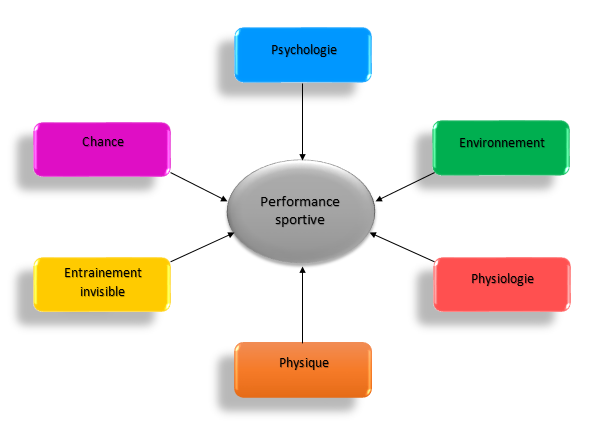
\includegraphics[scale=0.69]{images/facteursPerf}
            \caption{\label{fig:facteursPerf}Facteurs de la performance en athlétisme}
        \end{figure}
        
        
        \subsection{Facteurs physiologiques}
        
        Les facteurs physiologiques sont les éléments qui permettent de rendre visible la partie invisible de la performance dans le sens où l'étude de ces facteurs permet de comprendre le fonctionnement d'un organisme. Pour un entraîneur, l’étude de la physiologie sportive peut notamment lui permettre d'élaborer des entraînements adaptés au comportement physiologique de l'athlète. Plus précisément, cela permet d'étudier l’adaptation du corps à l'effort au niveau des systèmes nerveux et de l'organisation mécanique et physique de l'athlète, mais aussi au niveau biochimique, cardio-vasculaire et respiratoire.\\
        
        Dans l'expérimentation (\autoref{part:experimentation}), nous nous intéresserons à cette dernière partie et plus particulièrement à l'analyse de la glycémie, de la lactatémie, de l'oxymétrie de pouls et de la fréquence cardiaque.\\
    
    
        \subsubsection{La glycémie}
        \label{glycemie}
        
        La glycémie correspond au taux de glucose (ou taux de sucre) contenu dans le sang sachant que le glucose est la principale source d'énergie de notre organisme. La glycémie oscille en permanence en fonction du moment de la journée, des efforts physiques réalisés et surtout de l'alimentation, mais toute variation importante de celle-ci influe sur le bon fonctionnement du corps. Il est alors important que la glycémie demeure constante et modérée, c'est à dire comprise entre 3,5 mmol/l (63 mg/dl) et 6,1 mmol/l (110 mg/dl) de sang à jeun et inférieure à 7,8 mmol/l (140 mg/dl) deux heures après un repas. \\

        Lorsque le taux de sucre dans le sang est trop faible (inférieur à  63 mg/dl), on parle alors d'\textbf{hypoglycémie} (fatigue, sensation de malaise). Il suffit d'ingérer une dose de glucides (sucre par exemple) pour que la machine reparte dans les minutes qui suivent. Si ce taux est supérieur à 63 mg/dl à jeun ou 140 mg/dl deux heures après un repas, on parle d'\textbf{hyperglycémie}. \\
        
        La glycémie est contrôlée pour maintenir un apport énergétique constant à tous les organes. Elle est régulée par l’action de nombreuses hormones qui peuvent être regroupées en deux groupes. D'une part, les hormones dites « anaboliques »  représentées par l’insuline, qui permet d'abaisser la glycémie, et d’autre part, les hormones antagonistes à l'insuline communément appelées « cataboliques », hormones de stress ou hormones de la contre-régulation à l’hypoglycémie. Celles-ci sont des hormones hyperglycémiantes c'est à dire qu'elles augmentent le taux de glucose dans le sang. Parmi elles, on retrouve le glucagon, l’adrénaline, les glucocorticoïdes et l’hormone de croissance.    \\

        Le taux de glucose dans le sang augmente lors des apports alimentaires pour diminuer petit à petit et retrouver une valeur normale quand les mécanismes de régulation se sont mis en place. Dans ce système régulateur complexe, l'insuline joue un rôle primordial, car elle permet de faire entrer le glucose dans les cellules et en cas d'excès, de diminuer la production de glucose par le foie. \\

        \label{ig}Chaque aliment possède un indice glycémique (IG), qui fait référence à la vitesse d'élévation de la glycémie qu'ils entraînent (taux de sucre dans le sang). Ils sont classés en trois catégories : 
        
        \begin{itemize}
            \item IG élevé : charge glycémique supérieure à 70 (farines blanches et céréales raffinées, sucreries, dattes, etc.);
            \item IG moyen : charge glycémique de 50 à 70 (céréales complètes, fruits secs, etc.);
            \item IG bas : charge glycémique inférieure à 50  (la plupart des fruits et légumes, légumineuses, riz brun, quinoa, etc.)\\
        \end{itemize}
        
        Dans le schéma ci-dessous (fig. \ref{fig:indice_glycemique}), nous pouvons constater que lors de l'ingestion d'un repas composé majoritairement d'aliments à indice glycémique bas (courbe verte), la glycémie reste constante jusqu'à 2 heures après le repas puis diminue progressivement. Par conséquent, la consommation d'aliments à IG bas est préconisée avant un effort, car cela permet une efficacité énergétique plus durable. A l'inverse, nous pouvons remarquer qu'après la consommation d'aliments à indice glycémique élevé (courbe rouge), la glycémie augmente brutalement et atteint un pic 30 minutes après l'ingestion. Elle diminue ensuite tout aussi brutalement et l'athlète se retrouve en état d'hypoglycémie 2 heures après le repas. Ces aliments sont alors déconseillés comme dernier repas avant un effort, mais ils sont utiles juste après. En effet, étant donné qu'ils augmentent instantanément la glycémie, ils facilitent la récupération rapide.
        
        \begin{figure}[H]
            \centering
            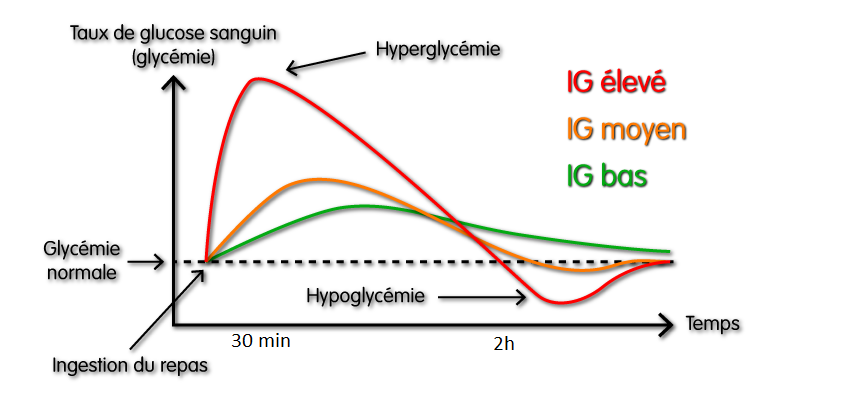
\includegraphics[scale=0.6]{images/courbe-index-glycemique.png}
            \caption{\label{fig:indice_glycemique}Mécanisme de l'indice glycémique}
        \end{figure}
        
        
        \subsubsection{La lactatémie}\label{lactatemie}
        
        La lactatémie représente la concentration de lactate dans le sang. Elle est généralement mesurée en exprimé en millimoles de glucose par litre de sang (mmol/l). \\

        Le lactate est un sel majoritairement produit par les muscles, les globules rouges et les cellules cérébrales au cours de la production d'énergie anaérobie (sans oxygène). Il participe à la production énergétique dont les muscles ont besoin pour fonctionner, mais il peut également entraîner des conséquences importantes lorsqu'il est produit en quantité excessive.\\

        Au repos, en temps normal, le sang humain contient une faible concentration de lactate (1 à 2 mmol/l). Toutefois, lors d'un effort intense, les muscles sont soumis à une demande énergétique importante et la succession de contractions y limite la circulation sanguine. Les muscles sont alors moins oxygénés, mais continuent d'utiliser du glucose pour fonctionner.
        Lorsque les cellules musculaires ne sont plus suffisamment oxygénées, voire totalement privées d'oxygène, la consommation de glucose des muscles devient alors supérieure à l'apport d'oxygène dont ils bénéficient et le lactate est sécrété en quantité excessive.
        La mesure de la lactatémie permet ainsi de dépister une mauvaise oxygénation des tissus.\\
      
        En athlétisme ce phénomène opère dans différentes disciplines, mais principalement pendant les courses de 400m, 800m et 1 500m, comme le montre le tableau ci-dessous (fig. \ref{fig:lactatemie}). En effet, c'est au cours de la récupération de ces courses que la concentration de lactate sanguin est la plus importante.
        
         \begin{figure}[H]
            \centering
            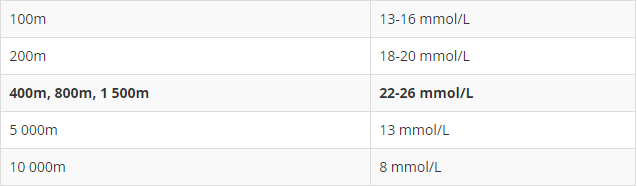
\includegraphics[scale=0.71]{images/lactatemie}
            \caption{\label{fig:lactatemie}Valeurs moyennes de lactatémie maximales chez des athlètes de haut niveau selon la discipline.}
        \end{figure}
        
        Ainsi, pendant un effort intense de plus de 20 secondes, la sur-production de lactate et de ce fait l’apparition de la fatigue musculaire est inévitable. Ceci se vérifie quel que soit le niveau de l'athlète.\\
        
        Le graphique ci-dessous (fig. \ref{fig:split_400}) décrit les temps de passage de chacun des 100m composant les records du monde du 400m de Michael Johnson en 1999 et plus récemment de Wayde Van Niekerk en 2016.\\
        
        
        \begin{figure}[H]
            \centering
            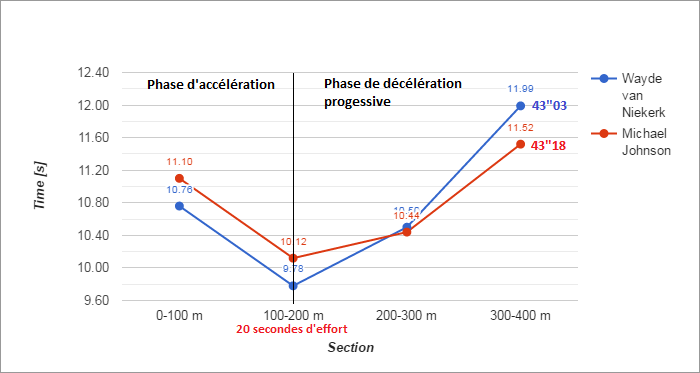
\includegraphics[scale=0.85]{images/split-times.png}
            \caption{\label{fig:split_400}Temps intermédiaires pour chaque 100m des records du monde de 400m}
        \end{figure}

        
        Nous pouvons clairement constater que pour les deux coureurs, les temps intermédiaires augmentent significativement dés 20 secondes d'effort. Le dernier 100m (dans la section 300-400m) est même couru plus de deux secondes plus lentement que le deuxième pour Van Niekerk et plus d'une seconde pour Johnson.\\
       
        L'objectif de l'entraînement sera donc de repousser au maximum la rencontre de cet épuisement.\\
        

        \subsubsection{L'oxymétrie de poul}
        \label{oxymetrie}
        
        L'oxymétrie de poul également appelée oxymétrie pulsée représente la quantité d'oxygène qui circule dans le sang et est déterminée par le niveau de saturation de l’hémoglobine en oxygène (SpO2). \\
        
        L’hémoglobine est une protéine contenue dans les globules rouges auxquels elle donne sa couleur. Elle est chargée de transporter l’oxygène dans le sang.\\
        
        Plus précisément, l'oxymétrie représente le pourcentage d’hémoglobine contenant de l’oxygène par rapport à la quantité totale d’hémoglobine dans le sang (hémoglobine oxygénée et hémoglobine non-oxygénée). \\
        
        La saturation pulsée de l’hémoglobine en oxygène est représentée par un pourcentage. Les valeurs normales de SpO2 sont situées entre 95 et 100\%. Si la valeur de la SpO2 est de 98\% cela signifie que chaque globule rouge présent dans le sang est composé de 98\% d’hémoglobine oxygénée et de 2\% d’hémoglobine non-oxygénée. Si la quantité d’oxygène distribuée par le sang aux tissus diminue et que la valeur de SpO2 est inférieure à 95\% cela peut être le signe d’une mauvaise oxygénation du sang aussi appelée hypoxie.\\

        Une bonne oxygénation du sang est importante pour fournir l’énergie nécessaire au fonctionnement des muscles et cela l'est d'autant plus lors d’une activité sportive. En effet, comme nous l'avons vu précédemment, une carence en oxygène entraîne une sur-production de lactate dans le sang et la difficulté de poursuivre un effort.\\
        
        
        \subsubsection{La fréquence cardiaque}
        \label{frequence_cardiaque}
           
        Le coeur est une pompe qui se contracte régulièrement pour assurer la circulation du sang à travers le corps, alimenter les muscles en oxygène et nutriments, mais aussi éliminer les toxines et déchets formés.\\
        
        La fréquence cardiaque correspond au nombre de contractions du coeur ou nombre de battements cardiaques par unité de temps (généralement évaluée sur une minute). Elle peut être mesurée sur plusieurs régions du corps comme le cou, le poignet, l’aine, le doigt ou encore le dessus du pied.
        Sa valeur au repos est généralement comprise entre 50 et 80 battements par minute (bpm) pour un sédentaire et entre 30 et 60 bpm pour un athlète.\\
     
        La fréquence cardiaque est une fonction linéaire du niveau d'effort fournit. Plus l'effort est intense, plus les besoins musculaires augmentent ainsi que les toxines évacuées. Le cœur doit alors battre plus rapidement pour pouvoir répondre à ces besoins. \\
        
        La mesure de la fréquence cardiaque peut être utilisée pour estimer en temps réel l'intensité de l'effort fournit. Sa valeur peut permettre de tester la forme de l'athlète grâce au calcul de la fréquence cardiaque au repos, du VO2max \footnote{Le VO2max ou consommation maximale d'oxygène correspond au volume maximal d'oxygène prélevé au niveau des poumons et consommé par les muscles par unité de temps.} et de la fréquence cardiaque maximale (FCM), mais aussi de gérer l'effort fourni. Après une course, l'exploitation de cette donnée peut permettre d'apprécier la capacité de récupération de l'athlète, mais également d'optimiser et de personnaliser les futurs entraînements. \\
    
        
        \subsection{Facteurs neuromusculaires et relatifs à la condition physique}
        
        Les facteurs neuromusculaires concernent la relation entre le système nerveux et le système musculo-squelettique. Ils permettent aux muscles de se contracter en fonction des différentes informations reçues.\\
        
        Ces facteurs sont généralement les plus complets et représentent les aspects de la performance qui occupent le plus grand degré de concentration et de temps de préparation. En effet, dans de nombreux sports, peu importe la façon dont l'athlète se consacre à l'entraînement, s'il n'est pas physiquement équipé pour concourir, la performance ne s'améliorera pas.\\
        
        La composante neuromusculaire de la performance sportive est subdivisée en ses propres éléments discrets qui doivent chacun faire l'objet d'entraînements spécifiques.\\
        
        Les entraînements principaux concernent :
            \begin{itemize}
                \item les filières énergétiques,
                \item la souplesse,
                \item la technique de course.\\
            \end{itemize}
        
        Ces entraînements sont influencés par l'anatomie de l'athlète et par la distribution de ses fibres. En effet, les muscles sont composés essentiellement de fibres musculaires.\\
      
        On compte principalement deux types de fibres musculaires :
        \begin{itemize}
            \item \textbf{les fibres rouges} (fibres lentes de type I) : peu de vitesse et peu de force, mais grande forte capacité de résistance à l’effort (endurance),
            \item \textbf{les fibres blanches} (fibres rapides de type II) : vitesse de contraction rapide et beaucoup de force, mais faible résistance à l’effort et incapables de se contracter longtemps (peu d'endurance).\\
        \end{itemize}
        
        C'est en fonction du type d'effort pratiqué que l'on utilisera l'une plutôt que l'autre (ou les deux) (fig. \ref{fig:fibres}).
        
        \begin{figure}[H]
            \centering
            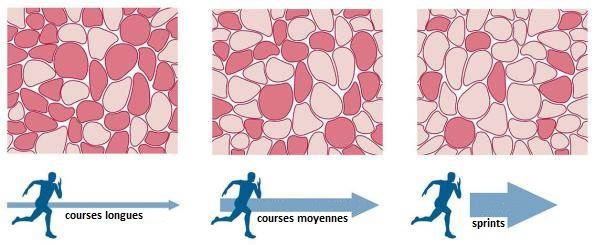
\includegraphics[scale=0.7]{images/fibres.jpg}
            \caption{\label{fig:fibres}Fibres sollicitées lors de différents types de courses}
        \end{figure}
        
        A la naissance, la composition des muscles est programmée génétiquement pour 50\%. Cela signifie que la moitié de nos fibres musculaires sera non modifiable et l’autre moitié sera transformable par l’entraînement.\\

        C'est donc en fonction des prédispositions génétiques de l'athlète, de ses aptitudes physiologiques et musculaires ainsi que de sa discipline que l'athlète va produire l'énergie nécessaire à l'accomplissement de son effort.\\
      
        Il existe trois modes de production d'énergie : 
        \begin{enumerate}
            \item la filière anaérobie alactique (sans oxygène et sans production de lactates),
            \item la filière anaérobie lactique (sans oxygène et avec production de lactates),
            \item la filière aérobie (avec oxygène).\\
        \end{enumerate}
        
        Chacune d’elle est caractérisée par une capacité (quantité totale d'énergie potentielle) et une puissance (quantité d'énergie délivrable par unité de temps). Par analogie avec un réservoir muni d'un robinet, la capacité correspond au volume du réservoir et la puissance au débit du robinet. 
        Bien que fonctionnant en parallèle, ces filières possèdent des durées de fonctionnement spécifiques qui les prédisposent à trois types d'efforts différents.\\
        
        \begin{description}
            \item  [La filière anaérobie alactique]
        est assurée par les fibres à contraction rapide des muscles. 
        Cette filière s’enclenche dès les premières secondes de l’exercice et est utilisée essentiellement dans les efforts réalisés au maximum d’intensité en un temps inférieur à 20 secondes. Toutefois, sollicitée à son maximum d’intensité, la filière anaérobie alactique est épuisée au bout de 7 secondes. En athlétisme les disciplines concernées par ce métabolisme énergétique sont les sprints explosifs tels que le 100 mètres.  Pour les courses plus longues (200 m, 400 m, 800 m), et les courses de haies (110 m haies et 400 m haies), le métabolisme anaérobie alactique est mis en jeu lors des 7 à 20 premières secondes, puis c'est la filière anaérobie lactique qui prend le relais.\\
        
        \item [La filière anaérobie lactique]
        se met en place lorsqu'il n’y a plus assez d’arrivée d’oxygène pour répondre à l’effort supérieur. Le corps fait alors appel à cette filière, qui consiste en une aide au fonctionnement du muscle. Toutefois, cette aide n’est pas sans conséquences. La filière anaérobie lactique utilise du glycogène, un sucre complexe présent à l'état de réserve au niveau du muscle, qui à la suite de réactions chimiques complexes, se transforme en lactate. L'accumulation de ces lactates dans le sang entraîne un apport d’acidité dans l’organisme qui perturbe la contraction du muscle.
        Résultat, la fatigue musculaire se fait sentir et la faculté de poursuivre son effort se réduit. \\
        
        Ce métabolisme s’enclenche dès les premières secondes de l’exercice, mais avec une intensité inférieure à celle du processus anaérobie alactique.
        Il assure des efforts de puissance élevée et de durée moyenne, de 20 à 45 secondes. C'est ce processus qui prédomine dans les courses de résistance comme le 400m ou le 400m haies.\\
        
        Le but de l’entraînement lactique est donc de produire beaucoup de lactate pour habituer l’organisme à ressentir la douleur, à la supporter pour ensuite repousser au maximum les limites de la tolérance. C'est ce qui permettra de retarder l'apparition de la fatigue musculaire.\\
        
        
        \item [La filière aérobie]
         représente les gammes d’intensité de travail d’endurance et est mis en place lors d'un effort long et modéré.
        Elle s'enclenche également dés le début de l'effort, mais c'est au bout de 3 minutes qu'elle devient la seule source d'énergie étant donnée que les deux autres ont été épuisées.
        La filière aérobie correspond à l’aptitude de l’organisme à capturer (respiration), transporter (globules rouges et débit cardiaque) et utiliser (efficacité oxydative des cellules) l’oxygène pour transformer l’énergie.
         
        C'est une qualité essentielle au succès quelle que soit la spécialité de l'athlète, car elle permet de régénérer les sources précédentes.\\
         
        Contrairement à ce que l'on pourrait penser, même dans les disciplines de courte durée et à haute intensité telles que le sprint par exemple, l'aérobie tient un rôle très important. Elle permet une meilleure oxygénation des muscles et participe à l’élimination des déchets de la contraction musculaire, ce qui favorise une récupération plus rapide et plus efficace après un entraînement ou une compétition. \\
        
        Dans les disciplines de fond, l'aérobie de l'athlète, c'est à dire sa capacité à consommer et traiter l'oxygène est primordiale. En effet, un des axes de travail du processus aérobie est de maintenir une intensité élevée le plus longtemps possible tout en dépensant le moins d'énergie possible.\\
        
        Cependant, ce processus n'est pas sans limite. 
        Lorsque l’athlète se rapproche du seuil critique du processus aérobie c'est à dire des limites pour lesquelles tout l’oxygène disponible au niveau musculaire est utilisé, on dit qu'il atteint son VO2max. \\
        
        Néanmoins, un athlète ayant atteint son VO2max peut encore augmenter l’intensité de son exercice. Ne disposant plus de réserves d’oxygène, il fera à nouveau appel à ses processus anaérobies, ce qui va provoquer une augmentation importante de la lactatémie. C’est le cas par exemple lors du sprint final d’un 1500m.\\
        
        \end{description}
     
         Dans le schéma ci-dessous (fig. \ref{fig:filieres-energetiques}), nous pouvons clairement voir que les trois sources ne sont pas indépendantes. Elles fonctionnent en parallèle, à des degrés divers, ce qui crée une illusion de fonctionnement en série. Pour chaque source, la surface comprise entre la courbe et l'axe du temps représente la capacité (l'endurance).\\
         
         \begin{figure}[H]
            \centering
            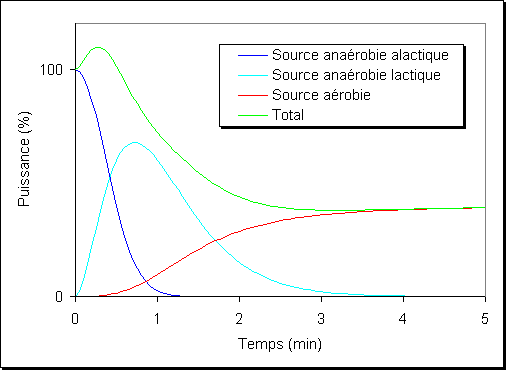
\includegraphics[scale=0.75]{images/aerobie-anaerobie-alactique2.png}
            \caption{\label{fig:filieres-energetiques}Les filières énergétiques}
         \end{figure} 
         
         
         La filière anaérobie alactique est celle qui produit le plus de puissance, mais qui a la plus faible capacité, c'est à dire qu'elle ne fournit pas d'énergie aux muscles longtemps : elle ne peut pas prolonger un effort à 100\% de son VO2max plus de 7 secondes. Au-delà de cette période, les muscles doivent utiliser d’autres procédés pour continuer la couverture énergétique. C'est le métabolisme anaérobie lactique qui prend le relais. Cette filière a une capacité et une puissance moyenne. Elle est active jusqu'à 3 minutes d'effort, mais produit une puissance élevée jusqu'à 45 secondes d'effort. Ensuite, la réserve d'énergie s'affaiblie et c'est la filière aérobie qui prend le relais. Ce métabolisme a une endurance très supérieure à celles des processus anaérobies, mais une puissance inférieure à celle assurée par ces derniers. A partir d'environ 3 minutes d'effort elle devient la seule source d'énergie et elle délivre sa puissance maximale vers 3 minutes 30 d'effort.\\
        
        La distribution des fibres à travers les muscles est donc régulée par la génétique, mais cette distribution n'est pas irréversible. Le but de l'entraînement est d'entraîner les fibres dans les filières énergétiques les plus importantes selon la spécialité de l'athlète pour maximiser leurs effets afin d'être le plus efficace possible. \\
        
        En plus des entraînements pour augmenter ses capacités énergétiques, l'athlète travaille aussi sa souplesse.\\
                

        \subsubsection{La souplesse}
        La souplesse désigne la qualité physique permettant d’accomplir des mouvements corporels avec la plus grande amplitude (articulaire et musculaire) et aisance possibles. que ce soit d’une manière active (en mouvement dynamique) ou passive (sans mouvement dynamique).\\
    
         On peut distinguer différents types de souplesse :
         \begin{itemize}
             \item la souplesse générale : mobilise les systèmes musculaires et articulaires pour faire en sorte d’apporter une aisance gestuelle;
             \item la souplesse spécifique : se rapporte à un muscle ou une articulation spécifique (e.g., franchir des haies nécessite une grande souplesse au niveau des ischios jambiers);
             \item la souplesse statique et dynamique : résulte de la présence ou non d’un mouvement;
             \item la souplesse active et passive : concerne la souplesse statique, leur différence réside dans la présence ou non d’une contraction musculaire;\\
         \end{itemize}

        En athlétisme, la souplesse est une qualité essentielle. Plus l'amplitude de mouvement présente dans les articulations d'un athlète est grande, meilleure sera l’efficacité du geste et la capacité de mouvement dynamique.\\

        La souplesse se travaille grâce à des étirements.\\
        
        Il existe deux types d'étirements: 
        \begin{itemize}
            \item les étirements avant séance :  pour réveiller les muscles, mais aussi augmenter et faciliter les amplitudes articulaires et musculaires (allongement des tissus et des muscles) qui seront utilisés lors de l'effort;
            \item les étirements après séance : pour permettre aux muscles de récupérer, mais aussi de prévenir les blessures.
            Il s’agit ici de relâcher et de décontracter les muscles pour retrouver un degré de tonus musculaire presque similaire au début de l’effort.\\
        \end{itemize}
                

        \subsubsection{La technique}
        
        En athlétisme, la maîtrise technique est un aspect indispensable pour le haut niveau.\\
        
        Cela englobe :
        \begin{itemize}
            \item la qualité des gestes (placements du corps et des articulations),
            \item la précision technique (pose de pied sous le bassin par exemple),
            \item la vitesse d’exécution (qui dépend aussi de la qualité et précision des gestes),
            \item la capacité de coordination.\\
        \end{itemize}
        
        Généralement la technique n'est pas innée et se travaille grâce à la répétition et à des exercices spécifiques. Cependant, il n'y a pas une seule technique efficace et universelle, mais plutôt une technique adaptée à chaque athlète en fonction du type de corps et des capacités musculaires de chacun.\\
    
        Ces différents facteurs ne sont pas les seuls déterminants de la performance en athlétisme. Nous allons maintenant nous intéresser à d'autres facteurs tout aussi importants.\\
        
                
        \subsection{Facteur psychologique}

            Le contrôle mental et les aspects psychologiques associés à la performance sportive sont des éléments déterminants qui se reflètent dans le résultat final de l'effort de l'athlète.\\
            
            En athlétisme, on dit que le mental joue pour 70\% de la performance et le physique pour seulement 30\%. C'est entre autres lui qui sépare les athlètes qui réussissent de ceux simplement talentueux. \\
            
            Toutefois, les éléments mentaux du sport sont à bien des égards les plus difficiles à maîtriser. Ils requièrent habituellement un haut niveau de maturité et d'expérience athlétique pour aboutir à des résultats et avoir la capacité d'être performant le jour J.\\
            
            Il n'est en effet pas rare de trouver des athlètes extrêmement doué physiquement, mais qui sont incapables de gérer la pression et de maîtriser leurs émotions pendant une compétition. Nous pouvons prendre l'exemple de Marie-José Perec, athlète surdouée et multiple médaillée olympique dans les épreuves de 200 et 400m, qui avait précipitamment quitté les Jeux Olympiques la veille de sa course sans explications.\\
            
            Les capacités cognitives de l'athlète (intelligence, mémoire, langage) peuvent expliquer certains comportements, car elles sont directement impliquées dans le processus mental. Elles concourent à l’appréhension et au traitement des informations ainsi qu'à l’analyse des situations. Le fait d'avoir une grande puissance analytique permet à athlète de prendre le contrôle de ses émotions et ainsi rester calme en situation de stress ou sous pression.\\
         
            La maîtrise émotionnelle n'est pas le seul point important de la force mentale d'un athlète. En effet, la capacité du sportif à avoir confiance en soi ainsi que son aptitude à être persévérant pour poursuivre son objectif jusqu’au bout, quelles que soient les difficultés rencontrées, sont également des qualités primordiales.\\
            
            Enfin, une des clés essentielles du succès est d'avoir un désir de réussite hors du commun. C'est cette envie qui permettra à l'athlète d'accepter la souffrance tout en se faisant plaisir, de s'auto-motiver et de pouvoir se surpasser tant en compétition qu'à l'entraînement.\\
            
                
        \subsection{Facteur social}
            
            L'athlète est un compétiteur, mais aussi et avant tout, un être humain évoluant dans un environnement et un contexte social au quotidien.\\
            
            Nous pouvons définir l’environnement comme étant un ensemble de conditions et de processus, englobant le système « entraînement-compétition » et plus globalement, la vie de l'athlète. \\
            
            Cet environnement peut être : 
            \begin{itemize}
                \item matériel : piste par exemple;
                \item physique : conditions climatiques, altitude;
                \item sportif : logique de formation / compétition, catégories et niveaux des athlètes;
                \item fédéral : calendrier des compétitions;
                \item relationnel : dynamique au sein du groupe; d’entraînement, situation familiale, affective ou professionnelle, relation entraîneur/entraîné.\\
            \end{itemize}

            Les pensées, sentiments et comportements de l'athlète sont influencés par son environnement et notamment par la présence réelle, imaginaire ou implicite des personnes qui gravitent autour de lui. La relation entraîneur/entraîné est un des éléments, si ce n'est l'élément le plus important dans l'environnement d'un sportif. Elle est généralement basée sur une entente entre une personne qui veut atteindre des objectifs et un guide qui peut l’y amener. Ce lien repose donc sur un désir de performance et peut être de différentes natures : amical, mentor/athlète, fraternel, etc. Quelle que soit la nature de cette relation, l'athlète et l'entraîneur passent environ 4h à 5h par jour ensemble dans le but d'atteindre un objectif commun. La qualité de la communication et la confiance entre les deux individus sont donc des éléments indispensables et déterminants dans leur quête de la réussite.\\
            
            Dans cette relation, le rôle de l'entraîneur est primordial. C'est lui qui va organiser les entraînements afin de favoriser le développement des capacités de l'athlète et l'amener à l'accomplissement de ses objectifs. C'est donc un gestionnaire, mais pas seulement. L'entraîneur est la personne qui va inspirer confiance à l'athlète, le soutenir dans les moments de doutes et qui va l'aider à utiliser des ressources connues ou inconnues pour solutionner un problème. C'est aussi celui qui va aider l'athlète dans son développement personnel afin d'augmenter son bien-être au quotidien.\\
         
         
            L'environnement social de l'athlète module et influence donc l'organisation et la gestion des entraînements/compétitions, mais aussi leur réalisation.
            Cependant, les facteurs environnementaux sont rarement sous le contrôle personnel de l'athlète. La capacité de l'athlète à s'adapter à des facteurs environnementaux différents et inattendus est souvent déterminante pour la réussite. \\
            
            
        \subsection{Facteur chance}    
            
            Le facteur chance est un facteur qui peut être controversé, mais qui existe néanmoins. Il conditionne les éléments extérieurs et non contrôlables autour de la performance.\\
            
            Le facteur chance englobe :
            \begin{itemize}
                \item le nombre et le niveau des adversaires;
                \item les éventuelles blessures et abandons des adversaires;
                \item les erreurs de jugement (athlète disqualifié par erreur par exemple);
                \item la configuration des séries et des couloirs. Par exemple, en athlétisme et notamment aux 400m/400m haies, le couloir 1 est le pire couloir en terme de rapidité du fait de sa proximité avec le centre du stade et par conséquent, de ses virages serrés. Cependant, lors des séries, les couloirs sont tirés au  hasard et il est possible pour tous les athlètes de l'avoir. Un autre exemple ou la chance entre en jeu est lors de la configuration des couloirs par rapport aux concurrents : un athlète qui est au couloir 5 aura un avantage par rapport à celui qui est au couloir 6, car il bénéficiera du visuel sur lui. Il pourra ainsi le contrôler plus facilement et éviter des surprises;
                \item les conditions météorologiques. Ces conditions sont un facteur qui sera le même pour tous les concurrents. Il faudra alors avoir une meilleure capacité d'adaptation que les autres.\\
            \end{itemize}
            
            Pour un athlète cherchant à maximiser sa performance, il ne doit pas seulement exercer un contrôle mental pour éviter d'être dérangé par ces conditions, mais il doit également examiner les moyens de faire fonctionner les conditions dans le positif.\\
            
             
             
        \subsection{L'entraînement invisible}
         
            Chaque séance d’entraînement, chaque compétition provoque une dépense énergétique proportionnelle à l’intensité et la durée de la sollicitation musculaire. \\
             
            L'entraînement invisible correspond à optimiser tout ce qui tourne autour de l'entraînement physique pour rentabiliser au maximum ses effets. Il s’agit des domaines que l’on pourrait classer dans l’hygiène de vie et qui permettent d'optimiser la récupération. \\
            
            Concrètement, cela consiste à se préparer au mieux à l’effort, à optimiser son alimentation pour restaurer les réserves énergétiques et les tissus utilisés ainsi qu'à s'entretenir par des soins divers, tout cela pour éviter le surentraînement et prévenir l'apparition de blessures.\\
            
            Le surentraînement est un phénomène qui intervient lorsque la durée de récupération entre les séances n’est pas respectée ou mal gérée. Cela engendre une accumulation de la fatigue et une régression progressive des capacités physiques de l'athlète. Il est alors primordial de trouver le bon équilibre entre activité physique (entraînement, compétition) et récupération (repos, alimentation, soins, etc.). Cette phase de récupération va permettre à l'ensemble des systèmes sollicités pendant l’effort de se restructurer et de régénérer les réserves énergétiques.\\
              
            La récupération est donc l'une des clés de la performance.\\
    
            Les paramètres d'une bonne récupération sont : 
             \begin{itemize}
                 \item le sommeil,
                 \item les soins,
                 \item l'alimentation et l'hydratation.
                
             \end{itemize}
             
            Beaucoup d'athlètes négligent partiellement ou totalement l'entraînement invisible, pourtant il est tout aussi important que l'entraînement physique. \\
            
    
                \subsubsection{Le sommeil}
        
                    Il est reconnu qu’un manque de sommeil ou un sommeil perturbé peut nuire au fonctionnement mental et physique, affaiblir le système immunitaire et affecter les autres processus de rétablissement importants pour les athlètes.\\
                    
                    Un sommeil de qualité est alors indispensable pour un athlète. C’est pendant le sommeil qu’il y a une grande circulation des hormones de croissance et par conséquent une régénération des tissus cellulaires endommagés par l’entraînement. Il permet ainsi à l’organisme de récupérer des efforts qu’il a fourni. \\
                    
                    Une bonne nuit de sommeil se caractérise par :
                    \begin{description}
                        \item [Le besoin en sommeil.] La quantité de sommeil nécessaire diffère selon chacun, mais un athlète ne devrait pas dormir moins de 8 heures par nuit. Celle-ci peut être complétée si nécessaire par des siestes.
                     
                        \item [La qualité du sommeil.] Plusieurs athlètes dorment suffisamment d’heures,
                        mais leur sommeil est de mauvaise qualité. Le sommeil n'est alors pas aussi réparateur.
                        \item [Le moment du sommeil.] Chaque athlète présente un chronotype particulier (préférence de l’individu à réaliser une activité à certaines périodes de la journée plutôt qu’à d’autres) : certains sont matinaux et d'autres non. Les horaires d'entraînement doivent donc être synchronisés avec le rythme de l'athlète pour ne pas perturber son besoin en sommeil.
                        \item [Les habitudes de sommeil.] Il est important d'adopter des habitudes de sommeil pour favoriser la récupération. Par exemple, instaurer des heures de coucher avant minuit puisque celles-ci sont les plus «récupératrices».\\
                    \end{description}
                
        
                 
                \subsubsection{Les soins}
   
                Pour un athlète, le corps est l'élément indispensable à la réalisation de l’objectif qu’il s’est fixé. Cependant, les entraînements quotidiens malmènent les muscles, tendons, articulations, etc.  Il faut donc prendre soin de son corps et faire en sorte qu'il soit dans le meilleure état possible pour affronter les lourdes charges d'entraînements. Il faut également que l'organisme consacre toute son énergie à régénérer ses réserves au lieu de lutter contre les inflammations et les blessures.\\
                
                Pour cela, le sportif doit réaliser des soins qui permettront de prévenir les blessures ou de les traiter, mais aussi à récupérer (soins dentaires, podologie, ostéopathie, kinésithérapie, cryothérapie, étirements, massages, etc.).\\
                
            
                \subsubsection{L'alimentation et l’hydratation}
                
                    Le corps humain a besoin d’apports externes pour faire fonctionner l’organisme et créer de l’énergie. Ces apports proviennent de l'alimentation et de l'hydratation quotidienne et sont d'autant plus importants chez un athlète du fait de ses hautes dépenses énergétiques.
                    Ils doivent comblés quantitativement et qualitativement les dépenses énergétiques de l'athlète afin de reconstituer les stocks d'énergie perdus.\\
                    
                    Outre la quantité et la qualité des apports, la répartition quotidienne des prises alimentaires doit être respectée : l’organisme doit être suffisamment alimenté avant l'effort pour pouvoir être performant, mais aussi après pour restaurer ses réserves énergétiques et se réhydrater.\\
                    
                    Après un effort intense, l'athlète dispose d'une «fenêtre métabolique» qui correspond à un intervalle de temps pendant lequel les aliments ingérés sont assimilés plus rapidement. C'est le moment favorable pour rétablir le stock d'énergie, c'est à dire le stock de glycogène musculaire.\\
                    
                    Ce phénomène prédomine durant la première heure après l’effort et diminue rapidement. Si l'apport glucidique n'est pas absorbé par l'athlète dans les 4 heures suivant l'effort, il lui faudra 3 jours pour récupérer à 100\%.
                    
                    \begin{figure}[H]
                        \centering 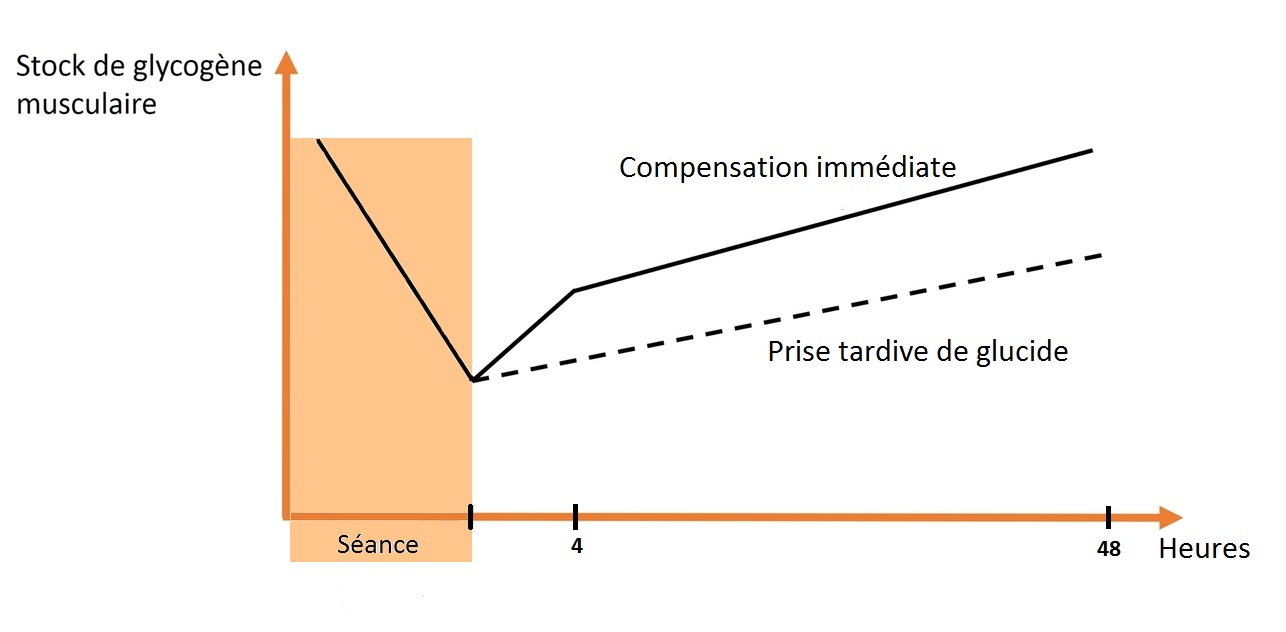
\includegraphics[scale=1.2]{images/fenetre-metabolique.jpg}
                        \caption{\label{fig:fenetre_metaboliques}La fenêtre métabolique}
                    \end{figure}
                    
                    
                    De la même façon, il est important d’assurer un bon équilibre hydrique en s'hydratant régulièrement, mais aussi d'adapter son apport en eau en fonction des pratiques en buvant avant, pendant et après l’effort. En effet, la transpiration et la sudation entraînent une perte d'eau supplémentaire. Lorsque la perte d’eau correspond à 2\% du poids de corps, la performance baisse de 20\%, si cette perte correspond à 4\% du poids de corps, à 18° de température ambiante la performance baisse de 40\%!  De plus, l'eau favorisera la restauration du stock minéral perdu et contribuera à diminuer l’acidité musculaire dû à l'effort.
    
              \vspace{20pt} 
             

        La performance est donc un système complet et organisé qui comprend une multitude de facteurs qui en sont les fondements. Ils se révèlent plus ou moins importants selon la situation, les caractéristiques de l’athlète et le contexte, mais ils doivent être connus et intégrés dans le processus d’entraînement afin de maximiser les performances de l'athlète et d'éviter fatigue et surentraînement. 


    
    

%%% Local Variables: 
%%% mode: latex
%%% TeX-master: "memoire"
%%% End:






        \chapter{Les outils de mesure de la performance}
\label{part:outils}

Après avoir étudié les facteurs de la performance en athlétisme, nous allons maintenant nous intéresser aux différents outils qui permettent de mesurer les facteurs physiologiques cités précédemment. \\

    \section{Lecteur de glycémie}
    
    Un lecteur de glycémie est un appareil permettant de mesurer la glycémie (cf. p.\pageref{glycemie}  \ref{glycemie}). Le taux y est affiché à l’écran et est exprimé en millimole de glucose par litre de sang, en milligramme de glucose par décilitre de sang (mg/dl) ou encore en gramme de glucose par litre de sang (g/l). \\
    
    Parfois, l’écran n’affiche pas de chiffres, mais seulement les mots « Low » ou « High », signifiant que le taux de glucose est trop faible ou trop élevé.\\
    
    Il existe deux systèmes de mesure du taux de glucose : 
    \begin{itemize}
        \item classique,
        \item en continu.\\
    \end{itemize}
    
    Les lecteurs de glycémie classiques et les systèmes de mesure du glucose en continu servent tout deux à évaluer le taux de glucose. Cependant, ces analyses ne proviennent pas des mêmes fluides corporels (fig. \ref{fig:capillaireVSinterstitiel}).\\
    
    Le glucomètre se base sur le glucose sanguin contenu dans les capillaires (figure B), c'est à dire les plus petits vaisseaux du corps humain, alors que les systèmes de mesure du glucose en continu ou systèmes de mesure de la glycémie interstitielle (figure A) se basent sur le glucose contenu dans le liquide interstitiel. Ce dernier est un liquide qui se trouve entre les cellules et les capillaires sanguins et dans lequel le glucose circule librement (fig. \ref{fig:capillaireVSinterstitiel}).
    
     \begin{figure}[H]
        \centering
        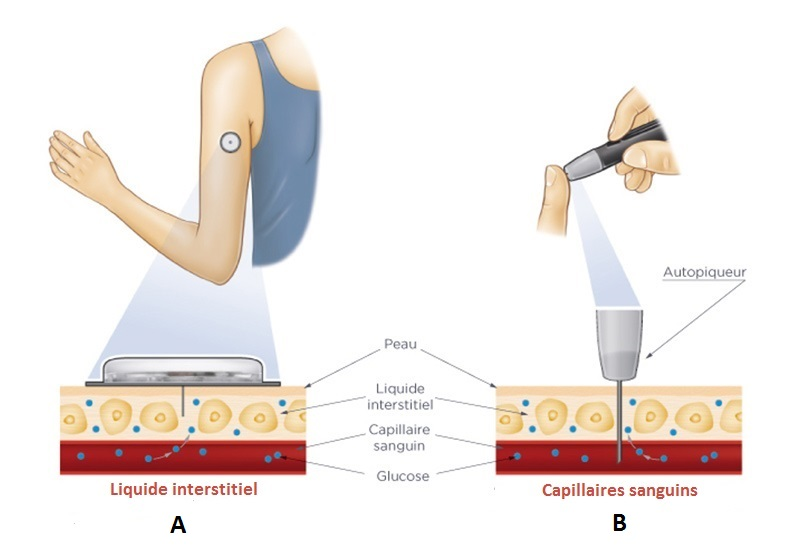
\includegraphics[scale=0.7]{images/glucometreVSfreestyle2.jpg}
        \caption{\label{fig:capillaireVSinterstitiel}Différents types de mesure de la glycémie. Glycémie interstitielle en continue (figure A), glycémie capillaire classique (figure B). }
    \end{figure}
    
    
    La glycémie capillaire est la méthode la plus utilisée et nécessite l'utilisation d'un auto-piqueur (muni d'aiguilles à usage unique appelées lancettes), de bandelettes et d'un lecteur de glycémie. \\
    
    Un petit échantillon de sang est prélevé et déposé sur la bandelette puis analysé par le glucomètre (fig. \ref{fig:glycemieCapillaire}).
    
    \begin{figure}[H]
        \centering
        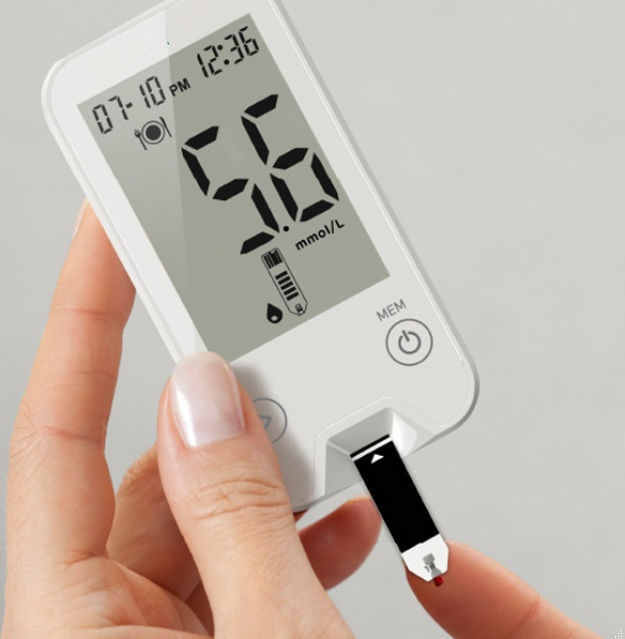
\includegraphics[scale=0.25]{images/glucometre.jpg}
        \caption{\label{fig:glycemieCapillaire}Système de mesure de la glycémie capillaire}
    \end{figure}

    
    Un système de mesure du glucose en continu est composé d’un capteur posé à l'arrière du bras pendant 14 jours et d'un lecteur qui permet de scanner le capteur et de collecter les données (fig. \ref{fig:systemeContinu}).
    
    \begin{figure}[H]
        \centering
        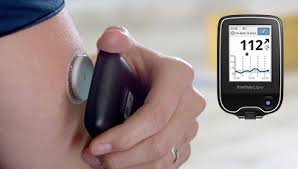
\includegraphics[scale=0.8]{images/glucometre2.jpg}
        \caption{\label{fig:systemeContinu}Système de mesure du glucose en continu}
    \end{figure}
    
    
    Les études ont montré que la quantité de glucose dans le milieu interstitiel reflétait le taux de glucose dans le sang, mais avec un décalage de quelques minutes (au maximum 10 minutes) dans certaines situations:
    \begin{itemize}
        \item lorsque la glycémie est en train de baisser,
        \item lorsque la glycémie est en train d'augmenter.\\
    \end{itemize}
    Ce décalage est principalement lié au temps de transfert du glucose entre le sang et le liquide interstitiel.\\
    
    Après une course, nous nous trouvons justement dans une de ces situations, car la glycémie se modifie. Un système de mesure de la glycémie interstitielle n'est alors pas adapté pour les athlètes qui souhaitent connaître leur glycémie immédiatement après un effort. Par conséquent, nous utiliserons un glucomètre classique pour l'étude de la glycémie dans le \autoref{part:experimentation}.
    
    
    \vspace{10pt}
    
    
    \section{Lactatomètre}
    
    Un lactatomètre est un appareil permettant de mesurer la lactatémie (cf. p.\pageref{lactatemie}  \ref{lactatemie}). Elle est exprimée à l'écran en millimoles par litre de sang (mmol/L).\\
    
    Les lactatomètres nécessitent l'utilisation d'un auto-piqueur pour le prélèvement du sang sur l'index ou le lobe de l'oreille de l'athlète ainsi que de bandelettes réactives, c'est à dire recouvertes d'une substance utilisée pour produire une réaction chimique. \\
    
    Un petit échantillon de sang est prélevé et déposé sur la bandelette puis analysé par le lactatomètre.\\

    Un des outils les plus répandus dans le monde du sport est le « Lactate Pro 2 » (fig. \ref{fig:lactatePro2}), car les résultats obtenus avec celui-ci sont aussi précis que ceux obtenus sur des appareils plus sophistiqués. 
    
     \begin{figure}[H]
        \centering
        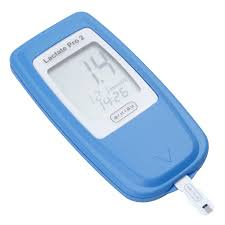
\includegraphics[scale=0.6]{images/lactatePro.jpg}
        \caption{\label{fig:lactatePro2}Lecteur de lactatemie « Lactate Pro 2 »}
    \end{figure}
    
    Le Lactate Pro 2 mesure le taux de lactate en seulement 15 secondes par prélèvement d'une très faible quantité de sang (volume d‘échantillon d'uniquement 0,3 \si{\micro}l). Le sang est automatiquement aspiré par la bandelette, ce qui réduit le risque d'erreur et garantit une mesure fiable sans contamination. \\
        
    De plus, toutes les données peuvent être transmises et archivées vers un PC de façon structurée grâce à l'interface USB intégrée. \\
    
    C'est cet outil que j'utiliserai dans le \autoref{part:experimentation}.\\
    
    
    \section{Oxymètre de pouls}

    L'oxymètre de pouls ou saturomètre est un appareil destiné à mesurer la fréquence cardiaque et l'oxymétrie de pouls (cf. p.\pageref{oxymetrie}  \ref{oxymetrie}). Il se présente généralement sous la forme d'un pince à doigt avec un capteur à l'intérieur et un écran qui affiche la saturation pulsée de l’hémoglobine en oxygène (SpO2) (fig \ref{fig:oxymetre}).
    
    \begin{figure}[H]
        \centering
        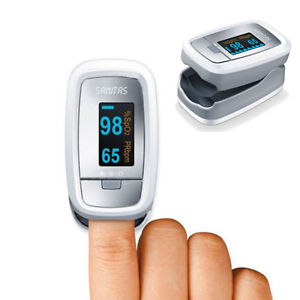
\includegraphics[scale=0.55]{images/oxymetre2.jpg}\hfill
        \caption{\label{fig:oxymetre}Oxymètre de pouls}
    \end{figure}
    
    L'avantage de cet outil est qu'il ne fait appel à aucun prélèvement sanguin.\\
    
    L'oxymètre de poul repose sur le principe d'absorption de la lumière c'est-à-dire sur la quantité de lumière absorbée pour une longueur d'onde donnée.
    L'émetteur de l'oxymètre émet deux faisceaux de lumière (rouge et infrarouge) de longueur d'onde différente (respectivement de 660 et 940 nm) à travers la peau et qui sont réceptionnés par un récepteur (fig \ref{fig:oxymetre_fonctionnement}).
    
     \begin{figure}[H]
        \centering
        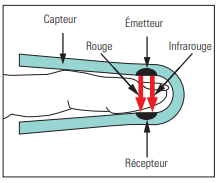
\includegraphics[scale=1]{images/oxymetre3.jpg}
        \caption{\label{fig:oxymetre_fonctionnement}Fonctionnement de l'oxymètre de pouls}
    \end{figure}
    
    L’hémoglobine riche en oxygène (oxyhémoglobine), absorbe la lumière infrarouge et laisse passer la lumière rouge alors que l’hémoglobine faible en oxygène (désoxyhémoglobine) absorbe la lumière rouge et est perméable à la lumière infrarouge. En calculant la différence d’absorption de ces deux lumières, l’oxymètre de pouls peut mesurer le niveau d’oxygénation du sang.

       
    \vspace{10pt}
     
    \section{Cardio-fréquencemètre}
    
        Le cardio-fréquencemètre est un outil incontournable du sportif, car il permet de mesurer instantanément sa fréquence cardiaque (cf. p.\pageref{frequence_cardiaque}  \ref{frequence_cardiaque}). \\
        
        Il existe des cardio-fréquencemètres avec ceinture thoracique et d'autres sans. 
        
        \subsection{Cardio-fréquencemètre avec ceinture thoracique}
        
            Le cardio-fréquencemètre avec ceinture (fig. \ref{fig:cardio_ceinture}) est généralement le plus utilisé et mesure l’activité électrique du coeur grâce à des électrodes qui permettent de capter les impulsions cardiaques. Les électrodes sont placées sur une ceinture émettrice positionnée sous la poitrine et qui est chargée de transmettre les données à un récepteur. Celui-ci est généralement porté au poignet sous forme de montre qui sert d'écran de contrôle et affiche la fréquence cardiaque.
            
            \begin{figure}[H]
                \centering
                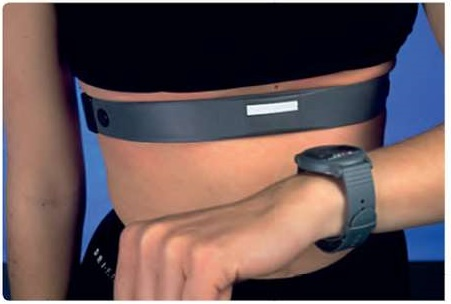
\includegraphics[scale=0.5]{images/cardio-ceinture2.jpg}
                \caption{\label{fig:cardio_ceinture}Cardio-fréquencemètre avec ceinture thoracique}
            \end{figure}
        
        Les cardio-fréquencemètres avec ceinture thoracique sont très performants et entièrement satisfaisants, mais le port d'une ceinture peut être contraignant pour un athlète. En effet, la ceinture peut gêner la respiration et certains athlètes peuvent développer des allergies au contact de celle-ci. Il arrive également que la fréquence cardiaque ne soit pas détectée en raison d'une trop faible humidification des électrodes ou d'un mauvais placement. De plus, des ondes circulent pour pouvoir transmettre les données entre la ceinture et le récepteur, ce qui n'est pas idéal d'un point de vue santé. Le signal peut également être parasité par d'autres ondes environnantes (lignes électriques, etc.). \\
        
        Il existe donc des cardio-fréquencemètres fonctionnant sans ceinture thoracique, qui sont moins encombrants et sans effet d'ondes puisqu'ils reposent sur une technologie complètement différente : la lecture optique.

         
        \subsection{Cardio-fréquencemètre sans ceinture thoracique}
         
        La lecture optique est la dernière technologie en matière de mesure de la fréquence cardiaque.
        Son principe de base est d'utiliser la lumière pour mesurer les variations de l'afflux sanguin engendrées par les battements du coeur. En effet, au moment du battement du coeur, la quantité de sang présente dans la zone testée est légèrement modifiée et le niveau de lumière change.\\
        
        Le capteur optique repose donc sur une source de lumière et un capteur de lumière. La source de lumière, composée d'une ou plusieurs LED, émet de la lumière qui va pénétrer les couches de la peau. Une partie de la lumière va être réfléchie et le capteur va réceptionner le signal lumineux. En analysant la quantité de lumière reflétée, le capteur sera capable de déterminer l’afflux sanguin et par conséquent, la fréquence cardiaque.\\
        
        Parmi les outils utilisables par le sportif, il existe la cardiobague qui se porte autour d'un doigt ou encore la montre avec cardio-fréquencemètre au poignet (fig. \ref{fig:cardiobague}).
        
         \begin{figure}[H]
                \centering
                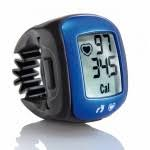
\includegraphics[scale=0.8]{images/cardiobague.jpg}
                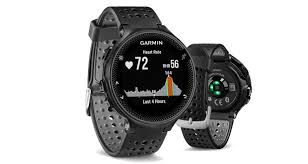
\includegraphics[scale=0.7]{images/garmin.jpg}
                \caption{\label{fig:cardiobague}Cardio-bague et montre cardio}
            \end{figure}


     En comparaison, il y a en moyenne 2 bpm d'écart entre les résultats obtenus par la mesure de la variation due au flux sanguin au bout du bras et ceux provenant de la mesure par impulsion électrique directement à la sortie du coeur. Étant donné que ces résultats sont très similaires, nous préférerons utiliser une montre cardio-fréquencemètre pour l'étude (\autoref{part:experimentation}).
        

   






    
        
%%% Local Variables: 
%%% mode: latex
%%% TeX-master: "rapport"
%%% End: 


        \chapter{Etat de l'art}
\label{part:etat_art}

Les relations qui peuvent exister entre la partie invisible de la performance et la performance elle-même ont suscité beaucoup d'intérêt. Voici un état de la littérature existante proposant des résultats intéressants et complémentaires à l'expérimentation qui va suivre.\\

La concentration sanguine de lactate est un des paramètres physiologiques qui a bénéficié du plus grand nombre d'articles de recherche, car la lactatémie est un des facteurs qui influence le plus la performance au 400 mètres.\\

   \section{Normes de la concentration de lactate}
       
       Selon l'étude de O. BANG \cite{bang36}, la concentration sanguine de lactate au repos est en moyenne de 1.94 mmol/l (fig. \ref{fig:lactate_repos}).\\
       
       \begin{figure}[H]
                \centering
                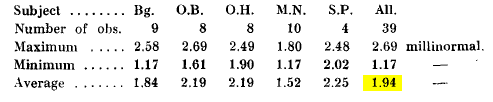
\includegraphics[scale=1]{images/lactate_repos.PNG}
                \caption{\label{fig:lactate_repos}Concentration sanguine de lactate au repos.}
        \end{figure}
        
       Pour F. PERONNET \cite{peronnet13}, les exercices courts et intenses comme le 400 mètres reflètent l'accumulation de grandes quantités de lactate qui peuvent avoisiner 30 mmol/l.
        
    \section{Effet de l'intensification de l'effort sur la lactatémie}
    
       Différentes études ont mis en évidence le fait que la lactatémie augmente progressivement au fur et à mesure que l'exercice s'intensifie.\\
       
       T. E.GRAHAM \cite{graham84} et A. P.CHASSAIN \cite{chassain86} ont tous deux étudiés l'évolution de la concentration du lactate sanguin lors de l'augmentation du pourcentage de V02max, c'est à dire à 60, 70 et 90\% de l'absorption maximale d'oxygène du sujet par exemple (fig. \ref{fig:lactate_vo2max}).\\
       
       \begin{figure}[H]
                \centering
                \fbox{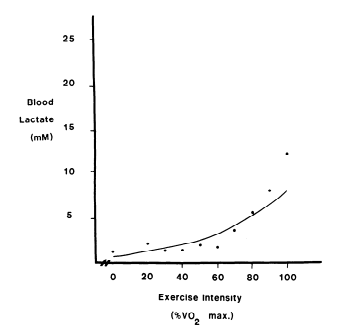
\includegraphics[scale=0.7]{images/lacta_vo2max.PNG}}
                \hfill
                \fbox{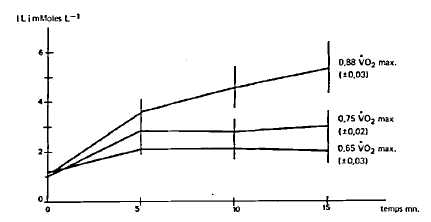
\includegraphics[scale=0.8]{images/lactate_vo2max3.PNG}}
                \caption{\label{fig:lactate_vo2max}
                La réponse du lactate sanguin à l'augmentation du pourcentage du VO2max. (Résultats de GRAHAM à gauche et CHASSAIN à droite).}
        \end{figure}
        
        T. E.GRAHAM et  A. P.CHASSAIN ont démontré que plus l'intensité de l'exercice augmente, c'est à dire que plus le sujet se rapproche de son VO2Max, plus sa concentration sanguine de lactate augmente. La lactatémie augmente significativement à partir de 60\% de la VO2Max.\\
      
       M. L. GOODWIN \cite{goodwin07} a quant à lui étudié l'évolution de la lactatémie lors de l'augmentation de la force générée c'est à dire du seuil de travail (calculé en watt) (fig. \ref{fig:lactate_work_rate}). L'exercice mis en place pour cette étude était de produire un effort de 4 minutes et d'augmenter l'intensité de 30W chaque minute. Les échantillons de sang étaient prélevés durant les 30 dernières secondes de chaque seuil de travail via un cathéter placé dans l'avant bras du sujet.\\
       
       \begin{figure}[H]
                \centering
                \fbox{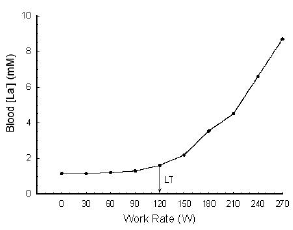
\includegraphics[scale=1]{images/lactate_work_rate}}
                \caption{\label{fig:lactate_work_rate}
                La réponse du lactate sanguin à l'augmentation du seuil de travail.}
        \end{figure}
        
        
        Enfin, dans leur étude, J. R. LACOUR et coll.\cite{lacour90} ont mesuré la lactatémie de 17 athlètes de haut niveau après des courses de 400 mètres. Les résultats qu'ils ont obtenus montrent que l'augmentation de la vitesse provoque également une hausse de la lactatémie (fig. \ref{fig:lactate_vitesse}).\\
    
          \begin{figure}[H]
                \centering
                \fbox{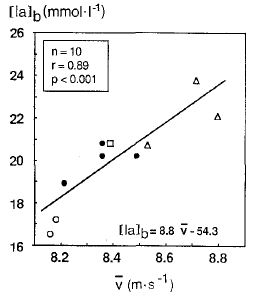
\includegraphics[scale=1]{images/lactate_vitesse}}
                \caption{\label{fig:lactate_vitesse}
                La réponse du lactate sanguin à l'augmentation de la vitesse.}
        \end{figure}
        
       
        Ainsi, quelque que soit la méthode utilisée, les recherches indiquent que la lactatémie augmente graduellement au début de l'exercice puis significativement lorsque l'effort devient plus intense. Ceci est expliqué par le fait que lors de l'exercice intense, ce sont les processus métaboliques anaérobies (sans oxygène) qui tiennent la place la plus importante. Le déficit en oxygène augmente donc progressivement, ce qui détermine une augmentation progressive de la concentration sanguine de lactate.\\

        
    \section {Lactatémie maximale après effort}
    
        Les résultats publiés par M. L. GOODWIN \cite{goodwin07} montrent que la concentration de lactate sanguin est la plus élevée dans les 3 à 8 minutes suivant la fin de l'exercice (fig. \ref{fig:lactate_recup}).
            
            \begin{figure}[H]
                \centering
                \fbox{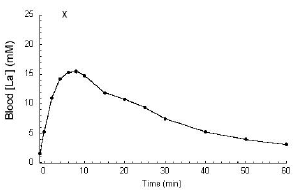
\includegraphics[scale=1]{images/lactate_recup}}
                \caption{\label{fig:lactate_recup} Évolution de la lactatémie après la fin de l'effort.}
             \end{figure}
            
        
        La plupart des études portant sur la lactatémie de fin de course ont été réalisées sur les disciplines de 400, 800 et 1500 mètres, car comme le montrent J.R LACOUR et coll.             \cite{lacour90}, ce sont elles qui mettent en jeu le métabolisme anaérobie lactique de façon la plus importante.\\
    
    
    \section{Lactatémie et performance}
        
        Dans la même étude, J.R LACOUR et coll. \cite{lacour90} se sont également attachés à déterminer s'il existait une relation entre la lactatémie et la performance, c'est à dire le temps réalisé au 400 mètres. Pour ce faire, ils ont mesuré la concentration sanguine de lactate à l'issue de courses de 400 mètres réalisées par des athlètes de niveau national et international lors de compétitions majeures comme les championnats de France, d'Europe et du Monde. Les échantillons ont été prélevés entre 5 et 10 minutes après la fin de l'effort et les résultats obtenus ont ensuite été mis en relation avec les meilleures performance de la saison de chaque athlète pour déterminer si une dépendance existait.\\           
        
        Les résultats montrent une corrélation systématique entre les performances réalisées et la concentration sanguine de lactate (r=0.89, P<0.01). Plus le temps réalisé par l'athlète se rapproche de sa meilleure performance de la saison, plus sa lactatémie augmente (fig. \ref{fig:lactate_velocite}). 
        
         \begin{figure}[H]
            \centering
            \fbox{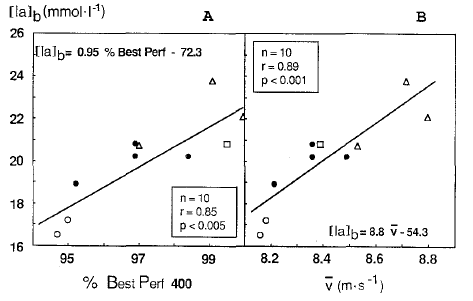
\includegraphics[scale=1]{images/lactate_velocite}}
            \caption{\label{fig:lactate_velocite} Évolution de la lactatémie post-effort.}
        \end{figure}
        
        Selon eux, les athlètes qui réussissent le mieux dans les exercices courts (de 10 secondes à 5 minutes) sont ceux qui produisent le plus de lactate et par conséquent, fournissent à leurs muscles le plus d’énergie par unité de temps. De la même façon, G.CAZORAL et coll. \cite{cazorla01} ont mis en évidence le fait que « ce n’est pas un hasard non plus si le guépard qui peut courir à 100 km/h est un très gros producteur de lactate ».  \\        
    

    \section {Fréquence cardiaque et SPO2}

        H. TABATABAEI \cite{tabatabaei00} s'est attaché à rechercher s'il existait une relation entre la SPO2 et la fréquence cardiaque.\\
        
        Les sujets de cette étude étaient une équipe national de canoe, de Taekwando, de lutte de des athlètes spécialistes des distances moyennes. Le test consistait à courir sur un tapis de course à la vitesse de 8 km/h au début, puis la vitesse augmentait de 1 km/h chaque minute jusqu'à épuisement. \\
        
        Les résultats indiquent que les deux variables sont bien corrélées, car plus la fréquence cardiaque est élevée, plus la saturation pulsée en oxygène est faible (fig. \ref{fig:spo2_fc}).\\
     
         \begin{figure}[H]
            \centering
            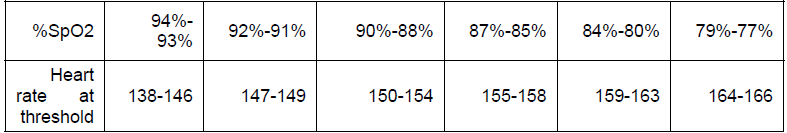
\includegraphics[scale=0.8]{images/spo2_fc.PNG}
            \caption{\label{fig:spo2_fc} Relation entre la fréquence cardiaque et la SpO2 pendant l'effort.}
        \end{figure}
        
        D. LAIN et coll. \cite{lain13} ont mené une étude similaire, mais à vélo, et ont observé qu'à partir d'une fréquence cardiaque environ égale à 170 bpm, la saturation pulsée en oxygène chute brutalement (fig. \ref{fig:spo2_fc2}.)
        
         \begin{figure}[H]
            \centering
            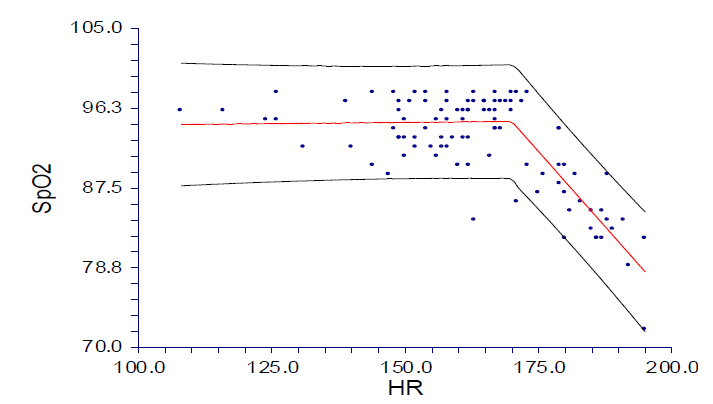
\includegraphics[scale=0.6]{images/spo2_fc2.PNG}
            \caption{\label{fig:spo2_fc2} Relation entre la fréquence cardiaque et la SpO2 pendant l'effort.}
        \end{figure} 
        

    \section{Étude de la glycémie après effort}
        
        Les effets d'un sprint court sur les taux de production et d'utilisation du glucose dans le corps a suscité plusieurs recherches.\\

        A.J. FAHEY et coll. \cite{fahey12} ont montré qu'un exercice maximal de seulement 10 secondes est capable de provoquer une augmentation des concentrations de glucose sanguin chez les individus en bonne santé (fig.\ref{fig:glycemie_posteffort}).\\
        
        \begin{figure}[H]
            \centering
            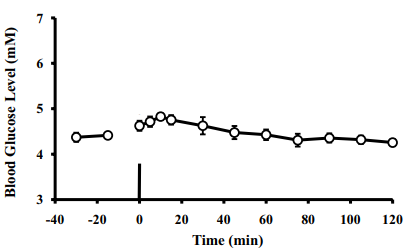
\includegraphics[scale=0.9]{images/glycemie_posteffort.PNG}
            \caption{\label{fig:glycemie_posteffort} Évolution de la glycémie en réponse à un sprint de 10 secondes (représenté par la barre verticale).}
        \end{figure} 

        Les résultats de l'étude effectuée par T.D. JUSTICE et coll. \cite{justice15} confirment ces résultats et indiquent que la glycémie augmente aussi après un sprint maximal de 30 secondes. Dans cette étude ils démontrent également qu'un exercice antérieur d'intensité modérée atténue l'effet d'augmentation de la glycémie d'un effort intense.
        
        \begin{figure}[H]
            \centering
            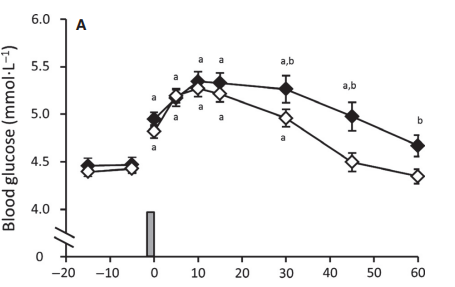
\includegraphics[scale=0.9]{images/glycemie_posteffort2.PNG}
            \caption{\label{fig:glycemie_posteffort2} Réponse de la glycémie à un sprint de 30 secondes (représenté par la barre verticale) réalisé après 60 minutes d'exercice d'intensité  modérée (losanges blancs) ou sans cet exercice (losanges noirs).}
        \end{figure} 
        
         Les niveaux de glycémie augmentent de manière significative et similaire dans les deux essais en réponse au sprint, atteignant un pic à 10 minutes de récupération. La glycémie a ensuite diminué plus rapidement lorsque que les sujets avaient effectué un exercice antérieur d'intensité modérée.


%%% Local Variables: 
%%% mode: latex
%%% TeX-master: "rapport"
%%% End: 

        
\chapter{Expérimentation et analyse}
\label{part:experimentation}

Maintenant que nous connaissons les facteurs qui influencent la performance ainsi que les outils qui permettent d'en mesurer certains, nous allons expérimenter ces outils sur des athlètes pour comprendre les facteurs qui influencent la performance.\\

Quatre aspects physiologiques différents seront mesurés après une course de 400m : la lactatémie, la glycémie, l'oxymétrie de pouls et la fréquence cardiaque. J'analyserai ensuite si les résultats obtenus permettent de comprendre la performance et de l'améliorer.\\
    
    
    \section{Méthodologie}
    \label{chap:methodo}

        \subsection{Sujets}
    
            Notre population d'étude est composée de 3 athlètes (homme n=1, femme n=2) spécialistes du 400m qui suivent tous un entraînement régulier dans le même club et avec le même entraîneur. Les caractéristiques de chacun d'eux sont présentées dans le tableau ci-dessous (fig. \ref{fig:tab-caracteristiques}).\\
            
              \begin{figure}[H]
                    \centering
                    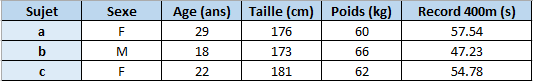
\includegraphics[scale=1]{images/tab_caracteristiques}
                    \caption{\label{fig:tab-caracteristiques}Caractéristiques des sujets}
                \end{figure}
            
            
            \subsection{Matériel}
            
                Pour réaliser l'étude le matériel suivant a été utilisé : 
                
                \begin{itemize}
                    \item un chronomètre manuel pour prendre le temps des athlètes lors la course de 400 m,
                    \item des gants en latex stériles,
                    \item des compresses stériles pour nettoyer le doigt des athlètes avant et après le prélèvement,
                    \item de l'alcool à 70°, pour nettoyer le doigt des athlètes avant et après le prélèvement,  
                    \item un stylo piqueur et des lancettes en métal, pour faire la piqûre au niveau de la pulpe du doigt et avoir un échantillon de sang à prélever,
                    \item des bandelettes de test Lactate Pro pour récupérer la goutte de sang,
                    \item un lactatomètre « Lactate Pro » de la marque ARKRAY pour mesurer la lactatémie,
                    \item un glucomètre pour mesurer la glycémie,
                    \item un oxymètre de poul de la marque Sanitas pour mesurer l'oxymétrie de pouls,
                    \item une montre Garmin Forerunner 235 pour mesurer la fréquence cardiaque.\\
                \end{itemize}
        
    
        \subsection {Déroulement des tests}
        
            L'objectif de notre travail est de comparer chez 3 athlètes la concentration sanguine de lactate (lactatémie), le taux de glucose sanguin (glycémie), la saturation pulsée en oxygène (oxymétrie de pouls) et la fréquence cardiaque avant et après une course de 400 m pour ensuite étudier les relations qui pourraient exister entre ces différents paramètres et enfin pouvoir comprendre la performance réalisée. \\
            
            Le plan expérimental se déroule sur 5 jours durant une semaine de stage où les trois athlètes sont dans les mêmes conditions : même alimentation, mêmes entraînements, mêmes heures de sommeil. \\
            
            Les tests ont eu lieu sur une piste d'athlétisme qui répond aux normes internationales de l'IAAF (Fédération Internationale d'Athlétisme). Elle se situe sur le stade municipal Romeo Neri à Rimini, en Italie.\\
            
            Les 3 sujets étaient répartis dans 3 groupes différents pour pouvoir effectuer les mesures chacun leur tour.\\
            
            Ils ont réalisé un 400 mètres à 12h30 les deux premiers jours du stage, puis ont eu un jour de repos et ont à nouveau réalisé un 400m les deux jours suivants.\\

            L'intensité du 400 mètres était maximale, c'est à dire qu'il était couru le plus rapidement possible, comme s'il était réalisé en compétition. \\
            
            Chaque course était précédée d’un échauffement d’une heure qui était le même pour les trois athlètes. L'échauffement été composé de 15 minutes de footing à une allure de 11 km/h, d'étirements, de gammes de course (talons fesses, montées de genoux, jambes tendus), de trois accélérations sur 80 mètres et enfin de trois départs en sprint sur 20 mètres.\\
            
            La saturation pulsée en oxygène a été mesurée avec l'oxymètre de pouls 2 minutes avant la course et juste après la fin de l'effort.\\
            
            La mesure de la fréquence cardiaque a été relevée sur la montre cardi-fréquencemètre 2 minutes avant la course et pendant la minute suivant l'arrêt de l'effort.\\
            
            Les échantillons de sang veineux pour la lactatémie et la glycémie ont quant à eux été prélevés  2 minutes avant la course et à partir de la 3ème minute de récupération.\\
            
            Avant le prélèvement, l'index de l'athlète était nettoyé avec une compresse et de l'alcool à 70°. La première goutte de sang qui apparaissait était aspirée par la bandelette du lactatomètre et la deuxième par celle du glucomètre.\\
            
            Le délai de prélèvement n'a jamais excédé 5 minutes.\\
         
            
            \subsection {Traitement statistique}
             
                Après avoir recueilli les données, ces dernières ont étés traitées grâce au logiciel de statistique R afin d'analyser l'existence ou non d'une relation entre lactatémie, glycémie, oxymétrie de pouls, fréquence cardiaque et la performance notamment. \\
                
                L'hypothèse posée est l'hypothèse nulle, ou H0, c'est à dire que les deux variables observées sont indépendantes.\\
                 
                Le rejet de l'hypothèse nulle implique donc l'existence d'une relation entre les deux variables observées.\\
    
                La prise de décision de rejet ou non de l’hypothèse nulle dépend de la probabilité de faire une erreur (p-valeur), c'est à dire de rejeter l'hypothèse nulle alors qu'elle est vraie. Nous appellerons la p-value p.\\
                
                La limite acceptable d'erreur a été fixée à 5\% (\si{\alpha}= 0,05).\\
                
                Nous dirons que:
                  \begin{itemize}
                      \item si la probabilité de faire une erreur (p-valeur) est inférieure à \si{\alpha} alors l'hypothèse H0 est rejetée et les variables sont dépendantes;
                      \item si la probabilité de faire une erreur (p-valeur) est supérieure à la probabilité \si{\alpha} alors l'hypothèse H0 est acceptée et les variables sont indépendantes.\\
                  \end{itemize}
              
                Pour mesurer l'intensité de la liaison entre les deux variables, le calcul du coefficient de corrélation, noté r, a été effectué. \\

                Le coefficient de corrélation est compris entre -1 et 1. Plus ce dernier est proche de -1 ou 1, plus la relation entre les deux variables est forte. On dit alors qu'elles sont fortement corrélées.\\
                
                Le coefficient est positif et la droite qui représente la corrélation est croissante si les deux variables ont tendance à augmenter ou à diminuer ensemble. Il est négatif et la droite décroissante si une variable a tendance à augmenter lorsque l'autre diminue.\\
                
                Un coefficient de corrélation nul signifie que les deux variables ne sont pas linéairement corrélées.\\ 
                 
                Pour résumé, en fonction du coefficient de corrélation, on dira que la relation entre les deux variables observées est :

                 \begin{figure}[H]
                    \centering 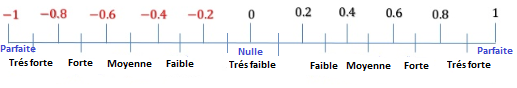
\includegraphics[scale=1]{images/coeff_corr}
                \end{figure}
            
 
              Enfin, pour être interprété, le coefficient de corrélation doit être significatif c'est à dire que la p-valeur doit être plus petite que le seuil fixé (ici 0,05).
 
 
    \section{Présentation des résultats}
    
        Toutes les données ont été stockées sous forme tabulaire dans des fichiers .csv et sont disponibles dans les Annexes (p.\pageref{annexe}).\\
        
        Les valeurs des variables biologiques qui ont étés analysées sont celles prélevées avant et après le 400 mètres, mais aussi l'écart entre ces deux mesures.\\
    
        \subsection{Fréquence cardiaque}
        \label{section:resfc}
        
        Les valeurs brutes de la fréquence cardiaque sont disponibles dans l'\autoref{annexe_fc}.\\
         
        Les graphiques ci-dessous (fig. \ref{fig:fc_perf_moy_seule}) présentent la relation entre la performance réalisée et la fréquence cardiaque avant le 400m puis après le 400m.\\ 
         
         \begin{figure}[H]
                \centering
                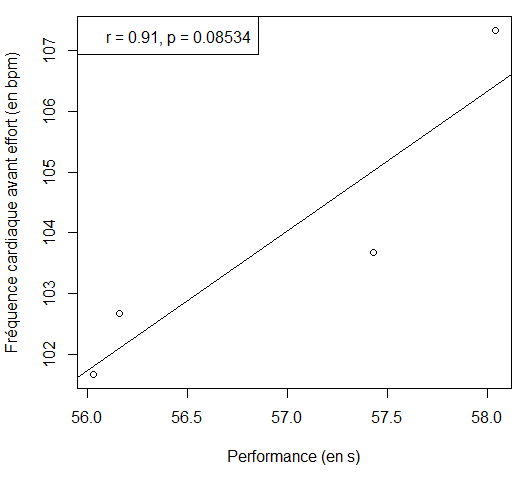
\includegraphics[scale=0.6]{images/fc_perf_av_moy_seule}
                \hfill
                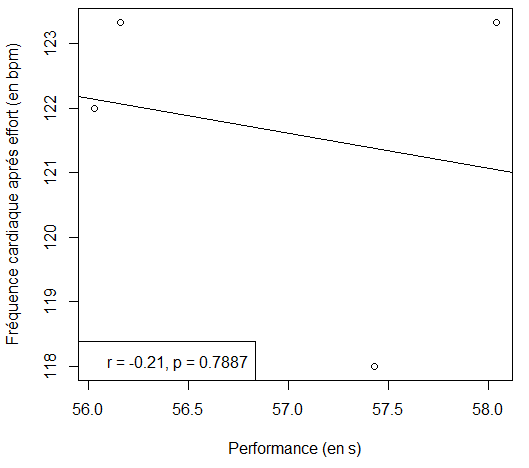
\includegraphics[scale=0.6]{images/fc_perf_ap_moy_seule}
                \caption{\label{fig:fc_perf_moy_seule}Relation entre la fréquence cardiaque avant la course (à gauche) et après (à droite) et la performance réalisée.}
            \end{figure}
            
          Les coefficients de corrélation trouvés indiquent qu'en moyenne il existe une relation très forte entre la fréquence cardiaque avant la course et le temps réalisé (r=0,91).\\
          
          Nous pouvons remarquer que la relation entre la fréquence cardiaque après la course et la performance est quant à elle très faible (r=-0,21).\\
         
 
         Enfin, les résultats présentés dans le graphique ci-dessous (fig. \ref{fig:fc_perf_ecart_moy_seule}) exposent une très forte relation (r=0,88) entre la performance réalisée et l'écart moyen de la fréquence cardiaque entre les valeurs avant un 400m et celles après .\\
         
         \begin{figure}[H]
                \centering
                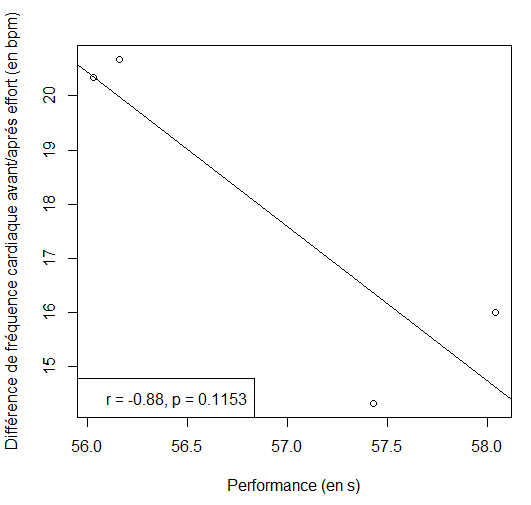
\includegraphics[scale=0.6]{images/fc_perf_ecart_moy_seule}
                \caption{\label{fig:fc_perf_ecart_moy_seule}Relation entre la performance réalisée et l'écart moyen de la fréquence cardiaque avant et après la course.}
            \end{figure}
            
            
        \subsection{Oxymétrie de pouls}
        \label{section:resOxy}
        
            Les valeurs brutes de l'oxymétrie de pouls sont disponibles dans l'\autoref{annexe_oxy}.\\
             
            Le tableau ci-dessous (fig. \ref{fig:oxy_recap}) présente les valeurs moyennes de l'oxymétrie de pouls en fonction de la performance réalisée par les trois sujets.\\
    
            \begin{figure}[H]
                \centering
                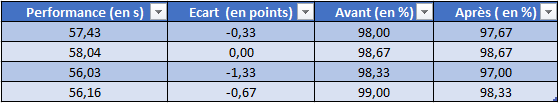
\includegraphics[scale=1]{images/oxy_recap}
                \caption{\label{fig:oxy_recap}Oxymétrie de pouls en fonction des performances réalisées sur les 4 jours de test par les 3 sujets.}
            \end{figure}
            
            Nous pouvons constater que les valeurs ne varient pratiquement pas. De ce fait nous ne pouvons pas supposer de relation particulière entre l'oxymétrie de pouls et la performance réalisée.\\
        
      
        \subsection{Glycémie}
        \label{section:resGlycemie}
        
            Les valeurs brutes de la glycémie obtenue sont présentées dans l'\autoref{annexe_gly}.\\
             
            Le graphique ci-dessous (fig. \ref{fig:gly_ecart}) décrit les écarts qui existent entre les valeurs de la glycémie avant le 400m et celles après. \\
            
            Nous pouvons remarquer que ces écarts sont toujours positifs c'est à dire que la glycémie est toujours plus élevée après le 400 mètres qu'avant.
    
            \begin{figure}[H]
                \centering
                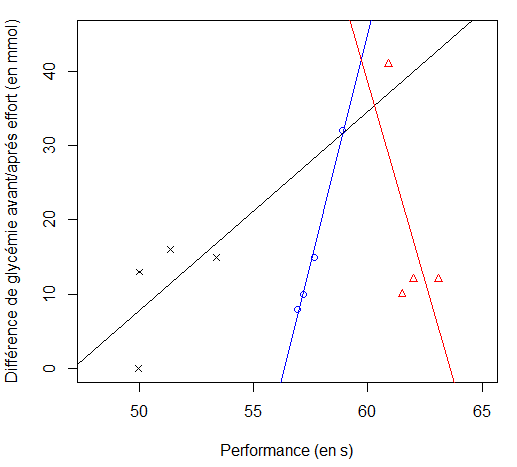
\includegraphics[scale=0.7]{images/gly_ecart}
                \caption{\label{fig:gly_ecart}Écart de glycémie entre les valeurs avant et celles après le 400m. Les symboles similaires font référence aux mêmes sujets.}
            \end{figure}
            
            
            Le graphique suivant (fig. \ref{fig:gly_perf_av}) présente la relation entre la performance réalisée et la glycémie avant le 400m.\\
            
            \begin{figure}[H]
                \centering
                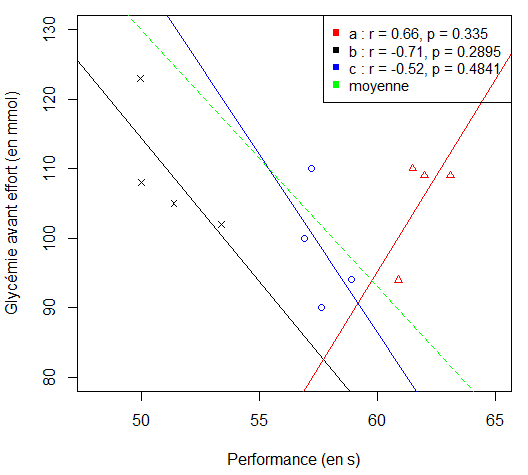
\includegraphics[scale=0.7]{images/gly_perf_av_moy}
                \caption{\label{fig:gly_perf_av}Relation entre la performance réalisée et la glycémie avant le 400m. Les symboles similaires font référence aux mêmes sujets.}
            \end{figure}
            
            Les coefficients de corrélation trouvés montrent qu'il existe bien une relation entre la performance et la glycémie avant la course pour les trois sujets (respectivement r= 0,66, r=-0,71 et r=-0,52). La moyenne indique une corrélation positive.\\
        
            Notons qu'aucun résultat intéressant n'a été trouvé concernant les valeurs de la glycémie après le 400m et la performance réalisée.\\
        
        
        \subsection{Lactatémie}
        \label{section:resLact}
        
            Les valeurs brutes de la lactatémie sont présentées dans l'\autoref{annexe_lact}.\\
            
            Les graphiques ci-dessous (fig. \ref{fig:lact_perf_av_ap}) présentent la relation entre la performance réalisée et lactatémie avant le 400m, puis après le 400m  pour chacun des sujets.\\
                   
            \begin{figure}[H]
                    \centering
                    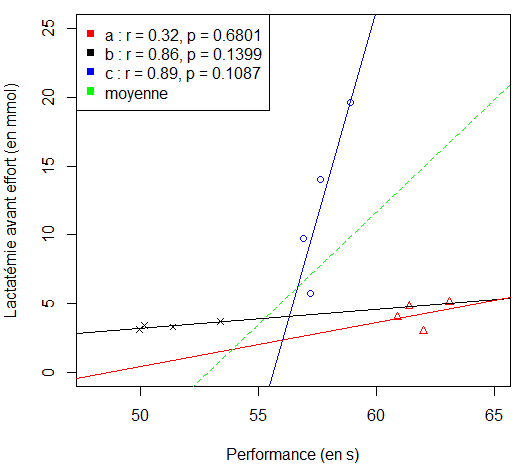
\includegraphics[scale=0.6]{images/lact_perf_av_moy}
                    \hfill
                    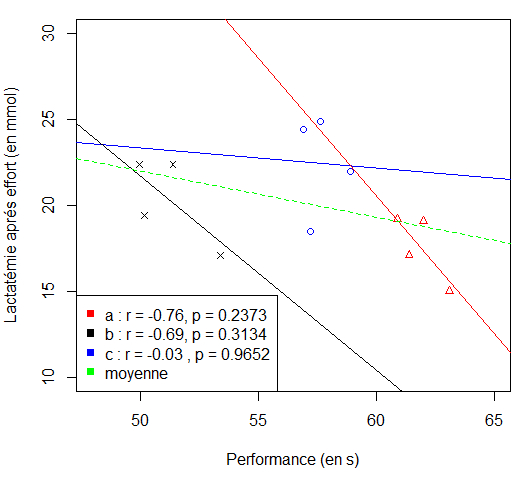
\includegraphics[scale=0.6]{images/lact_perf_ap_moy}
                    \caption{\label{fig:lact_perf_av_ap}Relation entre la performance réalisée sur une épreuve de 400m et la lactatémie avant la course (à gauche) et après (à droite). Les symboles similaires font référence aux mêmes sujets.}
            \end{figure}
            
            Au vue des coefficients de corrélation obtenus après les tests de régression linéaire, nous pouvons affirmer qu'il existe une relation entre la performance réalisée et la valeur de la lactatémie avant le 400m. La moyenne indique une très forte relation entre ces deux variables (r=0.84).\\
            
            Concernant la relation entre la performance réalisée et la valeur de la lactatémie après le 400m, la moyenne nous montre que la relation entre ces deux variables est faible (r=-0.29).\\
            
            Enfin, les résultats présentés dans le graphique ci-dessous (fig. \ref{fig:lact_perf_ecart}) montrent qu'il existe une forte relation entre la performance réalisée et l'écart de lactatémie entre les valeurs avant un 400m et celles après (respectivement r=-0,64, r=-0,71 et r=-0,997 pour les sujets a, b et c). La moyenne indique une très forte corrélation (r= -0.97) avec des résultats statistiquement significatifs (p=0.03).

                    
             \begin{figure}[H]
                    \centering
                    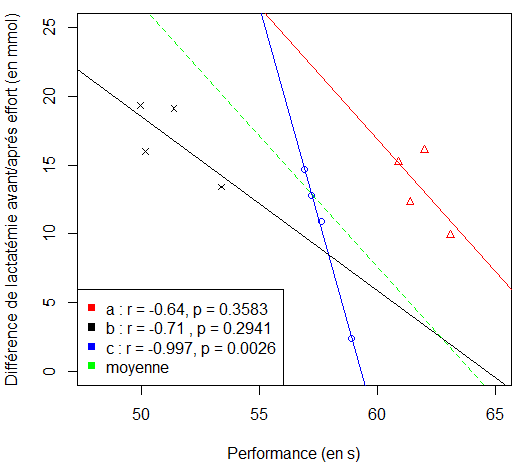
\includegraphics[scale=0.6]{images/lact_perf_ecart_moy}
                    \caption{\label{fig:lact_perf_ecart}Relation entre la différence de lactatémie avant et après le 400m et la performance réalisée. Les symboles similaires font référence aux mêmes sujets.}
            \end{figure}
        
        
    \section{Discussion}
    
        \subsection{La fréquence cardiaque et la performance réalisée}
        
        Les résultats que nous avons obtenus montrent qu'il existe une forte relation entre la performance et la valeur de la fréquence cardiaque avant un 400m. Nous remarquons qu'en moyenne, plus la fréquence cardiaque est faible avant la course, meilleur est le temps réalisé.\\
        
        De la même façon, la forte relation qui est exposée entre la différence de fréquence cardiaque avant et après la course et la performance réalisée indique que plus l'athlète est capable d'avoir une fréquence cardiaque basse avant le 400m et une fréquence cardiaque haute après, meilleure est la performance. \\
        
        En outre, les résultats montrent que la fréquence cardiaque après la course n'a pas vraiment de relation avec le temps réalisé. Cela peut être expliqué par le fait que la fréquence cardiaque dépend beaucoup des personnes. Certains ont une fréquence cardiaque qui augmente très rapidement après un exercice intense, mais ce n'est pas le cas pour d'autres.\\
        
        Je pense qu'il aurait été plus intéressant de mesurer la V02max pour connaître l'intensité de l'exercice effectué comme cela a été réalisé par A. P.CHASSAIN dans son étude \cite{chassain86}.
       

        \subsection{L'oxymétrie de pouls et la performance réalisée}
         
        Les résultats obtenus par la mesure de l'oxymétrie de pouls ne sont pas exploitables, car ils n'ont pas été fait dans les bonnes conditions. En effet, pour pouvoir observer des changements du taux d'oxygène dans le sang, il aurait fallu mesurer l'oxymétrie de pouls pendant l'effort. Cependant, cela demande du matériel que nous n'avions pas en notre possession, comme un masque de mesure d'oxygène par exemple.
         
         
        \subsection{La glycémie et la performance réalisée}
    
            La relation qui existe entre la glycémie avant la course et la performance réalisée indique qu'en moyenne, plus le taux de glucose sanguin d'un athlète avant le 400m est important, plus sa performance sera bonne par rapport à ses autres courses. Cela est cohérent : plus les muscles ont du glucose à disposition, plus ils pourront en consommer pour produire de l'énergie et finalement être plus efficace.\\
                
            Toutefois, l'augmentation de la glycémie avant une course ne peut pas être effectuée de la même façon suivant l'épreuve réalisée. Comme nous l'avons expliqué précédemment (cf. 1.2.1.\ref{ig}), les aliments n'ont pas tous le même indice glycémique et de ce fait la libération de l'énergie ne se fera pas dans les mêmes délais en fonction de l'absorption d'un aliment à IG bas, moyen ou élevé. L'ingestion d'un aliment à IG élevé moins de 30 minutes avant la course ne poserait pas de problème, voir pourrait être bénéfique pour un coureur de 400m, mais cela pourrait être risqué pour un coureur de 800m par exemple. Certes la première minute de course sera rapide du fait de la grande quantité de glucose et d'énergie disponible, mais très rapidement l'athlète se trouvera dans un état d'hypoglycémie du fait du manque de glucose qui aura été complètement utilisé. La fin de course s'avèrera donc compliquée.\\
                
            Concernant la glycémie après le 400m, la logique voudrait que celle-ci soit moins élevée qu'avant cet effort puisque pour assurer l'exercice, les muscles ont besoin d'énergie et consomment donc du glucose. Cependant, l'écart de glycémie entre la valeur d'arrivée et la valeur de départ est toujours positif ce qui indique que la glycémie est toujours plus élevée après le 400m qu'avant.\\
            
            Ces résultats étaient déjà ceux exposés par T.D. JUSTICE \cite{justice15}, mais se confirment dans la présente étude.\\
                
            Nous pouvons expliquer cela par le fait que lors d'une compétition ou d'un effort de courte durée, mais intense ou violent, l'athlète est généralement soumis au stress physique et/ou psychologique. Dans ce cas, le corps déclenche une augmentation des hormones de contre-régulation (cf. p.\pageref{glycemie}). Les hormones de stress ainsi sécrétées dans le corps provoquent la libération de sucre dans le sang et de ce fait une augmentation de la glycémie.\\
            
        
        \subsection{La lactatémie et la performance réalisée}
        
            
            Dans leur étude, J.R LACOUR et coll. \cite{lacour90} affirmaient qu'il y avait une forte relation entre la valeur de la lactatémie après un 400m et la performance réalisée (r=0.85). D'après eux, la concentration de lactate sanguin après une course était d'autant plus importante que l'athlète se rapprochait de sa meilleure performance de la saison. \\
            
            D'après mes résultats, il est vrai que la valeur de la lactatémie après le 400m est un indicateur important, mais ce n'est pas cette valeur qui explique la performance. En effet, elle ne signifie pas que plus la lactatémie est haute, plus l'athlète court vite, mais plutôt que plus la lactatémie est haute, plus l'athlète est \textbf{capable} de courir vite.  \\
            
            Comme l'a exposé F. PERONNET dans son étude \cite{peronnet13}, la concentration maximale possible de lactate est d'environ 30 mmol/l. Ainsi, si l'on remarque qu'a l'issue de chacune de ses courses un athlète n'atteint pas des valeurs de lactatémie élevées, c'est à dire que celles-ci ne dépassent jamais 20 mmol/l, cela signifie que l'athlète devra travailler sa capacité de production de lactate à l'entraînement pour augmenter ces valeurs. C'est précisément le cas du sujet A dans cette étude. De la même façon, même si un athlète présente des valeurs de lactatémie élevées (autour de 23 mmol/l), l'objectif de l'entraînement sera également d'augmenter sa capacité de production de lactate dans le but d'atteindre les valeurs maximales. \\
            
            La valeur de la lactatémie après le 400m est donc un indicateur de la capacité de production de lactate de l'athlète et par conséquent de sa capacité à courir vite, mais ce n'est pas elle qui explique la performance.\\ 
            
            J.R LACOUR et coll. ont obtenus de tels résultats, car ils se sont limités à la mesure de la lactatémie après effort et n'ont pas mesuré la concentration de lactate avant la course, ni l'écart qu'il pouvait exister entre la valeur d'arrivée et la valeur de départ de celle-ci.\\
            
            Typiquement, si nous prenons l'exemple du sujet C, la valeur de sa lactatémie après une course réalisée en 58,90s était de 22 mmol/l. Le sujet a ensuite réalisé une autre course en 57,21s et nous avons relevé une lactatémie après course de 18,5 mmol/l. Le fait que la lactatémie soit plus élevée lors de la course la plus lente confirme que ce n'est pas la forte production de lactate qui induit une meilleure performance. \\
            
            Ce phénomène s'explique ici par la valeur de la lactatémie avant le 400m. Celle ci était égale à 19,6 mmol/l lors de la première course et à 5,7 mmol/l lors de la deuxième. Il est logique que lorsqu'une course est débutée avec une lactatémie déjà élevée, cela engendre des valeurs plus élevées à l'arrivée.\\
        
            Les résultats obtenus par la présente étude ne sont donc pas en concordance avec ceux de J.R LACOUR et coll., car ils mettent en évidence le fait que ce n'est pas la valeur de la lactatémie après le 400 mètres qui est liée à la performance, mais plutôt l'écart observé entre la valeur de départ et la valeur d'arrivée de la lactatémie.\\
        
            Nous remarquons que pour un athlète, plus cet écart est important, meilleur est son temps réalisé par rapport à ses autres courses. Pour le sujet C, la corrélation entre l'écart de lactatémie avant et après le 400m et le chrono réalisé est pratiquement égale à 1 ce qui prouve une relation presque parfaite. L'écart de lactatémie serait donc un des points qui permettrait d'atteindre le meilleur niveau de performance pour un athlète.\\
           
            Il est néanmoins important de noter que cette observation ne peut pas être généralisée. Nous ne pouvons pas affirmer que plus la différence entre la lactatémie avant et après effort est grande, plus la performance réalisée est bonne. En effet, certaines variables de la composition corporelle comme le genre, le poids, le poids idéal, la masse graisseuse, etc ou même des éléments extérieurs comme le vent peuvent influer sur la production de lactate dans le sang. Par exemple, nous pouvons constater que le sujet C avait un écart de 2,4 mmol/l lorsqu'il a couru en 58.90s alors que le sujet A avait un écart de 16,1 mmol/l pour courir 3 secondes plus lentement (en 61.99s). Ceci signifie simplement que si le sujet C avait un écart plus grand, il courait plus vite. Cela est donc relatif à chaque athlète.\\
            
            Lors de l'analyse des données des deux premiers jours de l'étude, nous avons constaté des valeurs anormalement haute de la lactatémie avant le 400m pour le sujet C. En effet, celles-ci étaient égales à 19,6 mmol/l et à 14 mmol/l tandis que les sujets A et B avaient des valeurs proches de 3,5 mmol/l. L'écart entre les valeurs avant et après l'effort était donc faible et respectivement de 2,4 mmol/l et de 10,9 mmol/l.\\
            
            Nous avons alors décidé de modifier le protocole d'échauffement du sujet C pour analyser si ce dernier favorisait l'augmentation de la production de lactate dans le sang. Le sujet C devait alors réaliser le même échauffement que précédemment, mais l'avoir terminé 15 minutes avant le début de sa course et rester assis jusqu'à 1 minute avant sa course.\\
            
            Les résultats ont été sans appel. La lactatémie des deux jours suivant était égale à 5,7 mmol/l puis à 9,7 mmol/l ce qui a permis d'obtenir des écarts plus importants entre la valeur d'arrivée et la valeur de départ (respectivement de 12,8 mmol/l et de 14,7 mmol/l). Les performances se sont également largement améliorées passant de 58.90s et 57.65s les deux premiers jours, à 57.21s et 56.91s après la modification de l'échauffement.\\
            
            L'analyse de la lactatémie des sujets a donc été la mesure qui a permis de faire la découverte majeure de cette étude. Nous pouvons aujourd'hui avancer que l'une des clés de la performance au 400m est d'être capable de produire de grandes quantités de lactate tout en ayant des valeurs de lactatémie très basse avant la course. 

        
    \section{Menaces à la validité de l'étude}
        
        Il faut reconnaître que notre étude présente des limites. Une des menaces principale à la validité de cette étude est que l'échantillon observé (n=3) est trop petit. Cela pose problème, car la p-valeur est généralement supérieure au seuil fixé (\si{\alpha}= 0,05) ce qui montre que les résultats ne sont statistiquement pas significatifs. \\
        
        En outre, les mesures de la saturation pulsée en oxygène et de la fréquence cardiaque n'ont pas été effectuées de sorte à trouver des résultats intéressants. En effet, les mesures auraient du être prise pendant la course et non avant ou après. De cette façon nous aurions pu déceler des variations significatives et en tirer les conclusions qui s'imposent.\\
        

            
    \section{Perspectives}
        
        De multiples perspectives sont prévues pour cette étude. Tout d'abord l'étude va être poursuivie, mais avec un échantillon plus grand. L'objectif est d'avoir un échantillon composé de 10 à 15 sujets.\\
     
        Ensuite, la mesure de la fréquence cardiaque sera mesurée pendant l'effort grâce à un cardio-fréquencemètre qui enregistre les pulsations durant toute la durée de la course.\\
        
        Nous mesurerons également la VO2max, car cette valeur est un bon indicateur de l'intensité de l'effort produit. \\
        
        Par ailleurs, l'idéal serait d'obtenir un masque pour pouvoir mesurer le taux d'oxygène dans le sang pendant l'effort. \\
        
        Après avoir récolté ces données, cela pourrait être intéressant de mettre en relation la fréquence cardiaque recueillie pendant l'effort et la performance réalisée pour connaître les valeurs à partir desquelles la performance se détériore. De la même façon nous pourrons observer la VO2MAx et le taux d'oxygène dans le sang pour savoir à partir de quel intensité la quantité d'oxygène commence à diminuer. Ensuite, la lactatémie pourrait être mise en relation avec la SpO2 pour connaître le taux d'oxygène à partir duquel la production de lactate augmente significativement. \\
        
        Enfin, une suite de cette étude pourrait être d'intégrer des protocoles de méditation, d'hypnose ou de sophrologie dans le cadre de la préparation physique et mentale des athlètes afin évaluer les différences s'il y en a. Ces nouvelles démarches sont réputées pour aider l'athlète à se concentrer, à réduire le stress, mais aussi à mieux gérer la douleur. L'application de ces méthodes pourrait également avoir un effet sur les aspects physiologiques étudiés précédemment comme par exemple abaisser la fréquence cardiaque.\\
        
        L'objectif serait donc de voir à quel point l'esprit peut aider le corps dans la performance.
    
    

%%% Local Variables: 
%%% mode: latex
%%% TeX-master: "rapport"
%%% End: 

        \chapter*{Conclusion}
\addcontentsline{toc}{chapter}{Conclusion}
\markboth{conclusion}{conclusion}



TODO


%%% Local Variables: 
%%% mode: latex
%%% TeX-master: "memoire"
%%% End:

        \appendix  \label{annexe}
        

          \chapter{Données oxymétrie de pouls}
        \label{annexe_oxy}
        
        \begin{figure}[H]
            \centering
            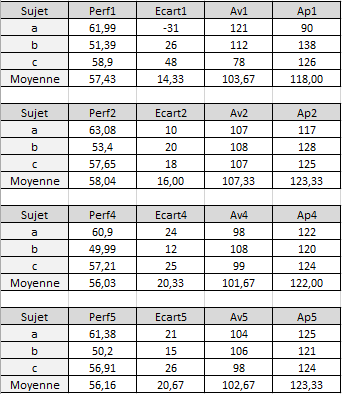
\includegraphics[scale=1.5]{images/donnees_fc}
            \caption{\label{fig:donnees_fc}Données brutes de la l'oxymétrie de pouls obtenue. « Perfn » correspond au temps réalisé le jour n, « Avn » à l'oxymétrie de pouls avant la course, « Apn » à l'oxymétrie de pouls après la course et « Ecartn » à la différence entre l'oxymétrie de pouls avant et après la course.}
        \end{figure}

        \chapter{Données fréquence cardiaque}
        \label{annexe_fc}
        
         \begin{figure}[H]
            \centering
            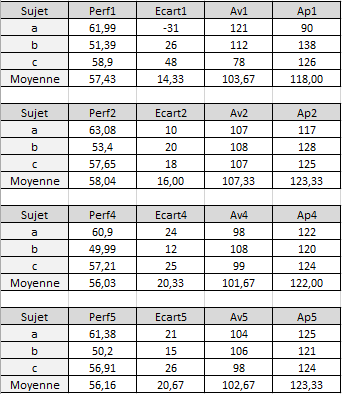
\includegraphics[scale=1.5]{images/donnees_fc}
            \caption{\label{fig:donnees_fc}Données brutes de la fréquence cardiaque obtenue. « Perfn » correspond au temps réalisé le jour n, « Avn » à la fréquence cardiaque avant la course, « Apn » à la fréquence cardiaque après la course et « Ecartn » à la différence entre la fréquence cardiaque avant et après la course.}
        \end{figure} 
        
        \chapter{Données glycémie}
        \label{annexe_gly}
        
         \begin{figure}[H]
            \centering
            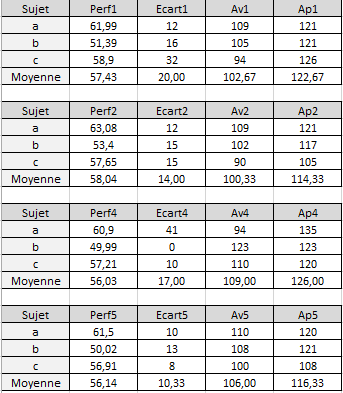
\includegraphics[scale=1.5]{images/donnees_gly}
            \caption{\label{fig:donnees_gly}Données brutes de la glycémie obtenue. « Perfn » correspond au temps réalisé le jour n, « Avn » à la glycémie avant la course, « Apn » à la glycémie aprés la course et « Ecartn » à la différence entre la glycémie avant et après la course.}
        \end{figure}
        
        \chapter{Données lactatémie}
        \label{annexe_lact}
        
        \begin{figure}[H]
            \centering
            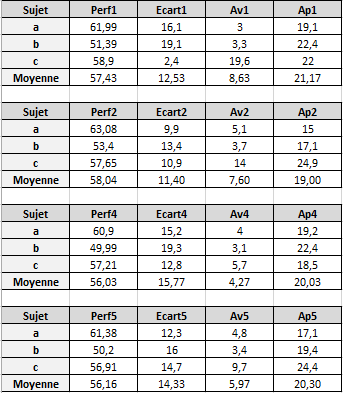
\includegraphics[scale=1.5]{images/donnees_lact}
            \caption{\label{fig:donnees_lact}Données brutes de la lactatémie obtenue. « Perfn » correspond au temps réalisé le jour n, « Avn » à la lactatémie avant la course, « Apn » à la lactatémie aprés la course et « Ecartn » à la différence entre la lactatémie avant et après la course. }
        \end{figure}
        
        \newpage
    
    \backmatter
        \nocite{*}
        \bibliographystyle{unsrt}
        \bibliography{references}    
        
        \newpage
        
        \renewcommand{\contentsname}{Table des matières}
        \setcounter{tocdepth}{6}
        \tableofcontents
    
 
\end{document}